%% abtex2-modelo-relatorio-tecnico.tex, v-1.9.6 laurocesar
%% Copyright 2012-2016 by abnTeX2 group at http://www.abntex.net.br/ 
%%
%% This work may be distributed and/or modified under the
%% conditions of the LaTeX Project Public License, either version 1.3
%% of this license or (at your option) any later version.
%% The latest version of this license is in
%%   http://www.latex-project.org/lppl.txt
%% and version 1.3 or later is part of all distributions of LaTeX
%% version 2005/12/01 or later.
%%
%% This work has the LPPL maintenance status `maintained'.
%% 
%% The Current Maintainer of this work is the abnTeX2 team, led
%% by Lauro César Araujo. Further information are available on 
%% http://www.abntex.net.br/
%%
%% This work consists of the files abntex2-modelo-relatorio-tecnico.tex,
%% abntex2-modelo-include-comandos and abntex2-modelo-references.bib
%%

% ------------------------------------------------------------------------
% ------------------------------------------------------------------------
% abnTeX2: Modelo de Relatório Técnico/Acadêmico em conformidade com 
% ABNT NBR 10719:2015 Informação e documentação - Relatório técnico e/ou
% científico - Apresentação
% ------------------------------------------------------------------------ 
% ------------------------------------------------------------------------

\documentclass[
	% -- opções da classe memoir --
	12pt,				% tamanho da fonte
	openright,			% capítulos começam em pág ímpar (insere página vazia caso preciso)
	oneside,			% para impressão em recto e verso. Oposto a oneside
	a4paper,			% tamanho do papel. 
	% -- opções da classe abntex2 --
	%chapter=TITLE,		% títulos de capítulos convertidos em letras maiúsculas
	%section=TITLE,		% títulos de seções convertidos em letras maiúsculas
	%subsection=TITLE,	% títulos de subseções convertidos em letras maiúsculas
	%subsubsection=TITLE,% títulos de subsubseções convertidos em letras maiúsculas
	% -- opções do pacote babel --
	english,			% idioma adicional para hifenização
%	french,				% idioma adicional para hifenização
	spanish,			% idioma adicional para hifenização
	brazil,				% o último idioma é o principal do documento
	]{abntex2}


% ---
% PACOTES
% ---

% ---
% Pacotes fundamentais 
% ---
\usepackage{lmodern}			% Usa a fonte Latin Modern
\usepackage[T1]{fontenc}		% Selecao de codigos de fonte.
\usepackage[utf8]{inputenc}		% Codificacao do documento (conversão automática dos acentos)
\usepackage{indentfirst}		% Indenta o primeiro parágrafo de cada seção.
\usepackage{color}				% Controle das cores
\usepackage{graphicx}			% Inclusão de gráficos
\usepackage{microtype} 			% para melhorias de justificação
% ---

% ---
% Pacotes adicionais, usados no anexo do modelo de folha de identificação
% ---
\usepackage{multicol}
\usepackage{multirow}
% ---

\usepackage{float}
% para posicionar a figura no local que tem interesse utilizando o "H"
% ou seja: \begin{figure}[H]
	
% ---
% Pacotes adicionais, usados apenas no âmbito do Modelo Canônico do abnteX2
% ---
\usepackage{lipsum}				% para geração de dummy text
% ---

% ---
% Pacotes de citações
% ---
\usepackage[brazilian,hyperpageref]{backref}	 % Paginas com as citações na bibl
\usepackage[alf]{abntex2cite}	% Citações padrão ABNT

% ---- Pacotes adicionados para PDF
\usepackage{pdfpages}

% --- 
% CONFIGURAÇÕES DE PACOTES
% --- 

% ---
% Configurações do pacote backref
% Usado sem a opção hyperpageref de backref
\renewcommand{\backrefpagesname}{Citado na(s) página(s):~}
% Texto padrão antes do número das páginas
\renewcommand{\backref}{}
% Define os textos da citação
\renewcommand*{\backrefalt}[4]{
	\ifcase #1 %
		Nenhuma citação no texto.%
	\or
		Citado na página #2.%
	\else
		Citado #1 vezes nas páginas #2.%
	\fi}%
% ---

% ---
% Informações de dados para CAPA e FOLHA DE ROSTO
% ---
\titulo{Relatório Técnico do Programa de Extensão: \\ Reciclagem Digital \\ Projetos: Manufatura Reversa, Hospital das Máquinas e Frankenstein}
\autor{Prof. Danny A.V. Tonidandel (DECAT) \\Prof. Cristiano L.T.F. e Silva (DEPRO) \\Profa. Regiane de S. e S. Ramalho (DECAT)}
\local{Brasil}
\data{2017}
\instituicao{%
  Universidade Federal de Ouro Preto - UFOP
  \par
  Departamento de Engenharia de Controle e Automação - DECAT
  \par 
  Departamento de Engenharia de Produção - DEPRO
  \par
  Pró-reitoria de Extensão - PROEX}
\tipotrabalho{Relatório técnico}
% O preambulo deve conter o tipo do trabalho, o objetivo, 
% o nome da instituição e a área de concentração 
%\preambulo{Modelo canônico de Relatório Técnico e/ou Científico em conformidade com as normas ABNT apresentado à comunidade de usuários \LaTeX.}
% ---

% ---
% Configurações de aparência do PDF final

% alterando o aspecto da cor azul
\definecolor{blue}{RGB}{41,5,195}

% informações do PDF
\makeatletter
\hypersetup{
     	%pagebackref=true,
		pdftitle={\@title}, 
		pdfauthor={\@author},
    	pdfsubject={\imprimirpreambulo},
	    pdfcreator={LaTeX with abnTeX2},
		pdfkeywords={abnt}{latex}{abntex}{abntex2}{relatório técnico}, 
		colorlinks=true,       		% false: boxed links; true: colored links
    	linkcolor=blue,          	% color of internal links
    	citecolor=blue,        		% color of links to bibliography
    	filecolor=magenta,      		% color of file links
		urlcolor=blue,
		bookmarksdepth=4
}
\makeatother
% --- 

% --- 
% Espaçamentos entre linhas e parágrafos 
% --- 

% O tamanho do parágrafo é dado por:
\setlength{\parindent}{1.3cm}

% Controle do espaçamento entre um parágrafo e outro:
\setlength{\parskip}{0.2cm}  % tente também \onelineskip

% ---
% compila o indice
% ---
\makeindex
% ---
% ----
% Início do documento
% ----
\begin{document}

% Seleciona o idioma do documento (conforme pacotes do babel)
%\selectlanguage{english}
\selectlanguage{brazil}

% Retira espaço extra obsoleto entre as frases.
\frenchspacing 

% ----------------------------------------------------------
% ELEMENTOS PRÉ-TEXTUAIS
% ----------------------------------------------------------
% \pretextual

% ---
% Capa
% ---
\imprimircapa
%

% ---
% Folha de rosto
% (o * indica que haverá a ficha bibliográfica)
% ---
\imprimirfolhaderosto*
% ---

% ---
% Anverso da folha de rosto:
% ---

{
\ABNTEXchapterfont

\vspace*{\fill}

\imprimirtitulo.

\begin{alineas}
  \item[*] Instituição: Universidade Federal de Ouro Preto $-$ UFOP;
  \item[*] Pró-reitotia de Extensão - PROEX; 
  \item[*] Programa de Extensão Reciclagem Digital;
  \item[] Coordenador do programa: prof. Danny Augusto Vieira Tonidandel; 
  \item[] Departamento de Engenharia de Controle e Automação;
  \item[] Unidade: Escola de Minas;
  \item[*] Ações Extensionistas: Manufatura Reversa, Hospital da Máquinas, Frankenstein;
  \item[] Modalidade: ações vinculadas ao programa;
  \item[] Coordenadores da ações: profa. Regiane S.S. Ramalho, prof. Cristiano L. T. F. Silva e prof. Danny A.V. Tonidandel $-$ 
  \item[] Departamentos: Engenharia de Produção (DEPRO) e Engenharia de Controle e Automação (DECAT);
  \item[] Unidade: Escola de Minas;
  \item[*] Período de Avaliação: abril a dezembro de $2016$;
  \item Número de alunos bolsistas: 6;
  \item Número de alunos voluntários: 0;  
  \item[*] Cidade: Ouro Preto $-$ MG $-$ Brasil;
  \item[*] publicação: Janeiro de $2017$;
\end{alineas}

\vspace*{\fill}
}

% ---
% Agradecimentos
% ---
\begin{agradecimentos}
Agradecemos à pró-reitoria de Extensão da UFOP, pelo fornecimento das bolsas para ações extensionistas, aos parceiros do programa, como o setor de desfazimento, da pró-reitoria de Administração (PROAD), bem como os doadores externos de peças e equipamentos.
\end{agradecimentos}
% ---

% ---
% RESUMO
% ---

% resumo na língua vernácula (obrigatório)
\setlength{\absparsep}{18pt} % ajusta o espaçamento dos parágrafos do resumo
\begin{resumo}
O programa \textbf{Reciclagem Digital}, ao qual os projetos \textbf{Hospital das Máquinas, Frankenstein e Manufatura Reversa} se vinculam, agrega ações que visam a diminuição do impacto ambiental provocado pelo lixo eletrônico que se desdobra em várias frentes, quais sejam, reforma e/ou atualização de computadores (hardware e software) de instituições envolvidas no programa, montagem de computadores a partir de material presente no descarte da UFOP e no aproveitamento de componentes eletrônicos a partir de eletroeletrônicos defeituosos coletados na comunidade. O programa tem caráter educativo, tanto na área socioambiental quanto econômico.

 \noindent
 \textbf{Palavras-chaves}: Reciclagem Digital. Educação Socioambiental. Inclusão Digital.
\end{resumo}
% ---
\cleardoublepage
% ---
% inserir lista de ilustrações
% ---
%\pdfbookmark[0]{\listname}{lof}
%\listoffigures*
%\cleardoublepage
% ---

% ---
% inserir lista de tabelas
% ---
%\pdfbookmark[0]{\listtablename}{lot}
%\listoftables*
%\cleardoublepage
% ---

% ---
% inserir lista de abreviaturas e siglas
% ---
%\begin{siglas}
%  \item[UFOP] Universidade Federal de Ouro Preto
%  \item[abnTeX] ABsurdas Normas para TeX
%\end{siglas}
% ---

% ---
% inserir lista de símbolos
% ---
%\begin{simbolos}
% \item[$ \Gamma $] Letra grega Gama
%  \item[$ \Lambda $] Lambda
%  \item[$ \zeta $] Letra grega minúscula zeta
%  \item[$ \in $] Pertence
%\end{simbolos}
% ---

% ---
% inserir o sumario
% ---
\pdfbookmark[0]{\contentsname}{toc}
\tableofcontents*
\cleardoublepage
% ---


% ----------------------------------------------------------
% ELEMENTOS TEXTUAIS
% ----------------------------------------------------------
\textual

% ----------------------------------------------------------
% Introdução (exemplo de capítulo sem numeração, mas presente no Sumário)
% ----------------------------------------------------------
\chapter{Introdução}
%
Segundo informações da Organização das Nações Unidas (ONU), o lixo proveniente de sistemas computacionais tais como computadores, celulares e similares cresce a uma taxa cerca de três vezes maior que a do lixo comum. Em pouco mais de $60$ anos após a aparição dos computadores no mundo, em que a obsolescência dos sistemas $-$ estimulada pelo consumismo das economias de mercado $-$ é cada vez mais precoce, a quantidade de lixo gerada a partir de componentes ainda em condições de uso é praticamente incalculável, assim como o impacto ambiental negativo que se converterá em pesado fardo para as gerações futuras. O lixo proveniente de materiais eletrônicos contém dezenas de contaminantes, como metais pesados e outros que, mesmo descartados de maneira correta (se encaminhados para aterros sanitários, por exemplo), podem provocar muitos danos ao meio ambiente. Entre as alternativas para se deter tal movimento, podemos citar o programa Universitária ``Reciclagem Digital'': idealizado por professores dos cursos de Engenharia de Controle e Automação e Engenharia de Produção da Universidade Federal de Ouro preto.

\section{Concepção do programa}
A ideia do primeiro projeto, que acabou se tornando o projeto ``Frankenstein'', surgiu a partir de uma demanda existente no laboratório de Instrumentação e Metrologia $-$ coordenado pela profa. Adrielle de Carvalho Santana e que possuía um monitor da disciplina de ``Metrologia Instrumentação'' (Gabriel) $-$. Havia uma necessidade de máquinas (leia-se computadores) para o referido laboratório. Na ocasião, a professora Adrielle e o referido aluno convidaram o prof. Danny Tonidandel e a profa. Regiane de S.S. Ramalho para fazerem uma visita ao setor de desfazimento da UFOP, em que observamos uma grande quantidade de peças e sistemas computacionais que estavam com o \textit{status} de ``obsoletos'' ou ``defeituosos''. A visão era impactante: pilhas e mais pilhas de computadores, monitores, teclados e impressoras, que tinham apenas um destino: o lixo.

No entanto, observamos rapidamente que diversos componentes eletrônicos, desde placas de circuitos, monitores e CPU's poderíam ser reaproveitados, não apenas para o laboratório de instrumentação, mas para auxiliar outras pessoas, já que grande parte seria simplesmente descartada pela universidade. Naquele instante surgiu a primeira ideia de se escrever um projeto de extensão, que seria mais tarde o Frankenstein.

Alguns dias depois da visita ao setor de desfazimento, durante um almoço no restaurante universitário, o professor Danny e a professora Adrielle conversavam sobre o tema e, tendo em mente o artigo $46$ do regimento da UFOP $-$ \textit{``A Universidade contribuirá, por meio de atividades de extensão, para o desenvolvimento material e cultural da comunidade''} $-$ pensamos que da área de descarte poderiam surgir outros projetos, que se transformariam no ``Manufatura Reversa'' e no ``Hospital das Máquinas'', que poderiam atender a uma maior parcela da comunidade, de maneira mais efetiva.

Assim, combinamos de não escrever apenas projetos isolados e sim um programa mais extenso, já que, por regra, um programa deve ter pelo menos dois projetos vinculados. No caso, tínhamos três, além de outros que ainda não saíram do papel. O programa então foi Batizado de Reciclagem Digital pela profa. Adrielle e  os projetos tiveram seus nomes escolhidos pelo prof. Danny, de forma a darem a ideia de seus objetivos:
\begin{itemize}

	\item Manufatura reversa: utilizar peças e componentes eletrônicos, a partir de itens descartados, para a criação de outros dispositivos, para atender à comunidade da ufopiana e externa, sendo que os componentes poderiam também ser coletados na comunidade externa. O ``manufaturas'' é o projeto que tem as metas mais ousadas para o futuro, em que se espera realizar a ``Mineração Urbana'', que consiste em retirar metais nobres (ouro, prata, platina) de componentes eletrônicos, a partir de um processo hidrometalúrgico. Esta função ainda está em processo de pesquisa;

	\item Frankenstein: montagem de computadores a partir de peças do setor de desfazimento da UFOP ou de doações externas;

	\item Hospital das máquinas: promover a manutenção regular (instalação de software e conserto de hardware) de computadores da comunidade (escolas, entidades sem fins lucrativos, etc.) como ferramenta promotora de educação e conscientização ambiental, com vistas à redução de lixo digital a partir do prolongamento de vida útil das máquinas. Este tinha também o caráter de fomentar a utilização de software livre e da filosofia \textit{Opensource} (GNU/Linux); 

\end{itemize}

Mais tarde, convidamos o prof. Cristiano L. T. de França e Silva, do DEPRO, por ser um grande entusiasta da filosofia do software livre e com experiência em gestão de projetos. A Equipe então estava formada e o programa começava a tomar forma, mesmo antes de ser submetido à PROEX.

Após o programa entrar em funcionamento, já na primeira semana, a Universidade recebeu uma grande doação de computadores descartados pelo Tribunal Regional do Trabalho de Minas Gerais (TRT-MG) e, o trabalho já se iniciou com uma grande demanda. A doação é creditada aos esforços do reitor, prof. Marcone Freitas junto ao TRT. O professor Marcone aliás, foi um dos maiores apoiadores do programa.

Desde o início, foi acertado que o objetivo do programa era, em essência, trabalhar pelo acesso às tecnologias digitais para uma maior inclusão social e educação: seja com o fornecimento de computadores, sua manutenção ou, simplesmente, pela retirada de lixo.

Assim, o programa esteve proibido, desde seu início, a prestar qualquer tipo de serviço a terceiros, como conserto de máquinas de departamentos ou unidades internas da UFOP, que são prerrogativa do NTI (Núcleo de Tecnologia da Informação). Assim, buscamos nos pautar pelos princípios que devem reger a vida do servidor público (o princípio LIMPE):`` Legalidade - Impessoalidade - Moralidade - Publicidade - Eficiência''.

Como o programa buscou trabalhar desde seu início de uma forma colaborativa e, de certa forma, interdependente, uma proposta inédita para organização foi pensada de forma a gerenciar suas atividades. A partir desta proposta surgiu um novo modelo de organograma, que chamamos de ``organograma orbital''.\footnote{Para mais detalhes sobre o modelo concebido, consulte o anexo \ref{ape:organograma}.}


\section{Justificativas}

Desde a concepção do Programa Reciclagem Digital, pôde-se observar um enorme intrelaçamento entre as três ações, sendo que o ``Hospital das Máquinas'' e o ``Frankenstein'' tornaram-se, rapidamente, os ``carros-chefe'' do programa. Daí mais uma razão para que o presente relato seja também unificado.


Na tabela \ref{tabela1}, apresenta-se um panorama os alunos participantes do programa ao longo do período.

\begin{table}[H]
\centering
\caption{Relação de alunos bolsistas e voluntários ao longo da realização do programa.}
\label{tabela1}
\begin{tabular}{|l|l|l|l|l|}
\hline
\textbf{Estudante} & \textbf{Matrícula} & \textbf{Admissão} & \textbf{Afastamento} & \textbf{Tipo} \\ \hline
Jonisson S. Santos & 14.1.1549 & 1/5/2016 & 31/12/2016 & Bolsista \\ \hline
Luciano E. de Almeida & 10.2.1179 & 1/5/2016 & 31/5/2016 & Voluntário \\ \hline
Gabriel V. R. Hoffman & 13.1.1656 & 1/5/2016 & 4/10/2016 & Bolsista \\ \hline
Heitor A. De Novais & 16.1.1397 & 11/10/2016 & 31/12/2016 & Bolsista \\ \hline
Aluizio J. Grecco & 14.2.1679 & 1/5/2016 & 31/12/2016 & Bolsista \\ \hline
Brian A. Fernandes & 13.1.1602 & 1/5/2016 & 31/12/2016 & Bolsista \\ \hline
\end{tabular}
\end{table}

\chapter{Objetivos}

O programa que abrange os projetos vinculados é, em essência o ``Rediclagem Digital'', coordenado atualmente pelo prof. Danny A. V. Tonidandel, do departamento de Engenharia de Controle e Automação (DECAT), tendo sido coordenado anteriormente pela profa. Adrielle de C. Santana, também do DECAT-EM-UFOP. O Reciclagem Digital buscou gerar, como produtos principais, computadores reciclados e novamente úteis à sociedade, peças reaproveitadas para as atividades de ensino e pesquisa na universidade, descarte adequado do ``lixo digital'' e, em especial, a conscientização das comunidades envolvidas na busca por um mundo mais limpo e equânime.

\section{Objetivos do ``Hospital da Máquinas''}
Consiste em estimular o uso destes sistemas por um período maior de tempo a partir de uma manutenção regular de hardware (futuro “lixo eletrônico”) e atualização software (futuro “lixo digital”), com a substituição de componentes defeituosos ou instalação/atualização de sistemas operacionais de fácil manutenção, de preferência software livre e de código aberto. Esta medida visa estender a vida útil das máquinas presentes na comunidade como agente promotora de educação no âmbito socioambiental, além de promover a diminuição da dispersão de material contaminante no meio ambiente. Muitas instituições possuem materiais eletrônicos parados que necessitam apenas de assistência técnica para terem perfeitas condições de uso. O projeto visa colocar para funcionar laboratórios de informática, com a instalação de softwares livres, juntamente com um pacote de programas e jogos educativos.

Coordenador: Prof. Cristiano L. T. de França e Silva.

\section{Objetivos do ``Manufatura Reversa''}
Promover o desmanche de equipamentos ditos "obsoletos", realizando o movimento inverso ao de uma linha de montagem. Separados, esses componentes (motores de passo, engrenagens, componentes eletrônicos etc) poderão, em tese, ser reaproveitados em outras aplicações, especialmente na educação e pesquisa na universidade. Esta medida visa auxiliar a comunidade a dar uma destinação útil aos componentes eletrônicos, tais como computadores, TV's celulares, aparelhos de som, bem como estimular a cultura do reaproveitamento, dado o alto valor agregado nos produtos eletrônicos.

Coordenador: Prof. Danny A. V. Tonidandel.

\section{Objetivos do ``Frankenstein''}
Realizar ações voltadas para a doação de computadores – recuperados a partir da área de descarte da UFOP – às instituições de ensino, arte, cultura, religiosas e/ou filantrópicas da região de Ouro Preto,  reaproveitando componentes e peças que viriam a contaminar o meio ambiente por meio de um descarte errôneo ou que continuariam ocupando espaço físico na universidade, além de promover a inclusão digital em instituições onde tais recursos são escassos.

Coordenadora: Profa. Regiane de S. e S. Ramalho.



\chapter{Métodos}

\section{Métodos do ``Hospital da Máquinas''}

Primeiramente foi feito um levantamento de instituições interessadas a participar do projeto através de um e-mail padrão desenvolvido pelos integrantes. Após definidas as instituições, foi marcada uma visita onde foi apresentado o projeto com a apresentação de um panfleto, sendo feito um levantamento do trabalho que seria, então, desenvolvido.

Durante o levantamento do trabalho desenvolvido, é costumeiro verificar o estado das máquinas e executar uma ou mais opções que seguem:

\begin{itemize}

	\item caso necessário é feito o reparo utilizando peças disponíveis no desfazimento;

	\item reinstalação do sistema operacional já disponível na máquina;
	
	\item formatação utilizando um sistema operacional Open Source distribuído gratuitamente, atualmente Linux Mint Xfce devido a simplicidade na utilização e exigir menos recursos das máquinas;
	
	\item desenvolvimento de um pacote de programas e jogos educativos para instalar nas máquinas, válido para todas as escolas;
	
	\item instalação de aplicativos adicionais sob demanda da instituição atendida;

\end{itemize}

Durante o trabalho de formatação e instalação de um sistema operacional livre, as máquinas são padronizadas com a instalação do sistema operacional Linux Mint. O trabalho é, normalmente, desenvolvido no próprio laboratório da escola. Após a realização do trabalho, a instituição assina um documento que comprova que os serviços foram prestados pelo projeto (vide anexo \ref{ordem-servico}.).

% Escola Estadual Dom Benevides
% Padronizar máquinas que já estão no laboratório com sistema operacional linux mint. 
% Verificar pentes de memória das máquinas já montadas, para aproveitar nas máquinas ociosas.
% Contabilizar quantas máquinas estão em uso, quantas foram padronizadas no novo sistema operacional.
% 8 máquinas estão ociosas, aparentemente por falta de memória.
%Casa Espirita Irmã Horta
%Necessita de doações para montar o laboratório. Ideia inicial da coordenadora é de 15 máquinas para compor o laboratório. Observar oferta e demanda de máquinas para ver a viabilidade disso.
%Inicialmente eles tem 2 máquinas DDR 3 e 1 monitor Philips preto funcionando e 2 notebooks.
%Foi recolhido 
%-1 notebook ITAUTEC INFOWAY W7635 
%-1 fonte output 20V
%-1 monitor defeituoso Philips Preto 166V3L5B/78
%Escola Estadual Dom Silvério
%Reativação do laboratório do Pronatec - 12 máquinas.
%Sala para alunos com necessidades especiais – 4 máquinas.
%Padronizar os computadores do laboratório do Pronatec com linux mint e instalar pacote educativo.
%Pesquisar programas para deficientes para instalar na sala para alunos com necessidades especiais.

\section{Métodos do ``Manufatura Reversa''}
A metodologia do ``Manufatura Reversa''consistiu basicamente em promover o desmonte de eletroeletrônicos defeituosos que seriam descartados por instituições da região para aproveitamento dos componentes eletrônicos como ferramenta promotora de educação e conscientização ambiental. Por isso tem igualmente caráter educativo na área socioambiental, além da técnica.

No início de suas atividades, a primeira etapa consistiu no cadastramento de instituições que desejavam ter materiais descartados, ou a partir de solicitações aos professores e bolsistas. Durante o cadastramento, ações informativas foram realizadas em relação ao processo
de manufatura reversa, que significa "desmontar para construir". Em seguida, o bolsista inicia a retirada dos equipamentos que seriam devidamente desmontados.

No caso das solicitações dos totens, das engrenagens entre outros, foram feitos testes em bancada e triagem dos subcomponentes advindos dos aparelhos eletrônicos, dos quais pode-se citar: engrenagens, capacitores etc. Após a triagem, teste e catalogação dos materiais, acondicionamento e posterior doação.

\section{Métodos do ``Frankenstein''}
O primeiro passo do projeto consistiu em selecionar bolsistas com conhecimento em manutenção de computadores para a realização dos trabalhos do projeto.
Para cada doação de um lote de computadores reciclados às instituições interessadas, foi realizada uma sequência de atividades.

A primeira atividade foi fazer um levantamento do lixo eletrônico existente nos setores da UFOP. A busca iniciou pelo Setor de Desfazimento, que havia recebido um grande volume de equipamentos de informática doados pelo Tribunal Regional do Trabalho (TRT). Dentre os equipamentos, haviam computadores, mouses, teclados, monitores, impressoras, cabos, etc. 

Uma análise de reaproveitamento do material encontrado foi realizada e os equipamentos que poderiam ser utilizados no projeto eram solicitados. O Setor de Desfazimento fazia uma consulta ao Núcleo de Tecnologia da Informação (NTI) da UFOP e, caso liberados pelo NTI, os equipamentos eram doados ao projeto. 

A segunda atividade foi fazer um levantamento das instituições interessadas em participar do projeto, recebendo doações de computadores reciclados conforme sua necessidade. Foram realizadas visitas a algumas instituições, onde foi apresentado o projeto e realizado o cadastro da instituição caso fosse do seu interesse.  

A terceira atividade foi fazer o transporte dos equipamentos do Setor de Desfazimento para o laboratório do Programa Reciclagem Digital, localizado na Escola de Minas do Campus Morro do Cruzeiro.
Em seguida, iniciou-se a manutenção dos computadores. Foram realizados testes no hardware das máquinas, troca de peças conforme necessidade, formatação e instalação de softwares básicos gratuitos, tais como sistemas operacionais baseados na plataforma GNU/Linux. Em seguida, as máquinas eram limpas, etiquetadas e embaladas para entrega. Foram confeccionadas etiquetas com a logomarca do Programa. O material utilizado para embalar as máquinas foram obtidos dentro da UFOP.

A etapa seguinte consistia em transportar as máquinas para a instituição que iria receber a doação. Ao chegar na instituição, as máquinas eram desembaladas, montadas e testadas. Algumas instruções básicas de uso foram passadas aos responsáveis, finalizando a doação. 

A última etapa consistia em transportar o lixo não aproveitado para o Projeto de Manufatura Reversa ou para instituições de reciclagem de metais, plástico e eletrônicos.

Reuniões, a princípio semanais e posteriormente quinzenais, eram realizadas com os bolsistas para orientações e para o bom funcionamento do projeto.
 
% ---
% Finaliza a parte no bookmark do PDF
% para que se inicie o bookmark na raiz
% e adiciona espaço de parte no Sumário
% ---
\phantompart

\chapter{Resultados}
Quando os primeiros equipamentos foram entregues pelo programa, o mesmo já era bem conhecido entre os docentes dos departamentos da Escola de Minas. Logo após, tivemos a honra da presença do Reitor da UFOP, o prof. Marcone, na primeira entrega. A cerimônia foi fotografada (Figura \ref{fig:entrega}) e , alguns dias depois, uma matéria foi veiculada na página principal da universidade, conforme pode-se consultar no anexo \ref{apendice:materia}, com grande repercussão na comunidade universitária e fora dela. Após a matéria, uma chuva de solicitações, bem acima da capacidade do programa, começou a acontecer, evidenciando a importância de programas deste tipo para a formação de uma sociedade mais justa. 

\begin{figure}[H]
	\centering
	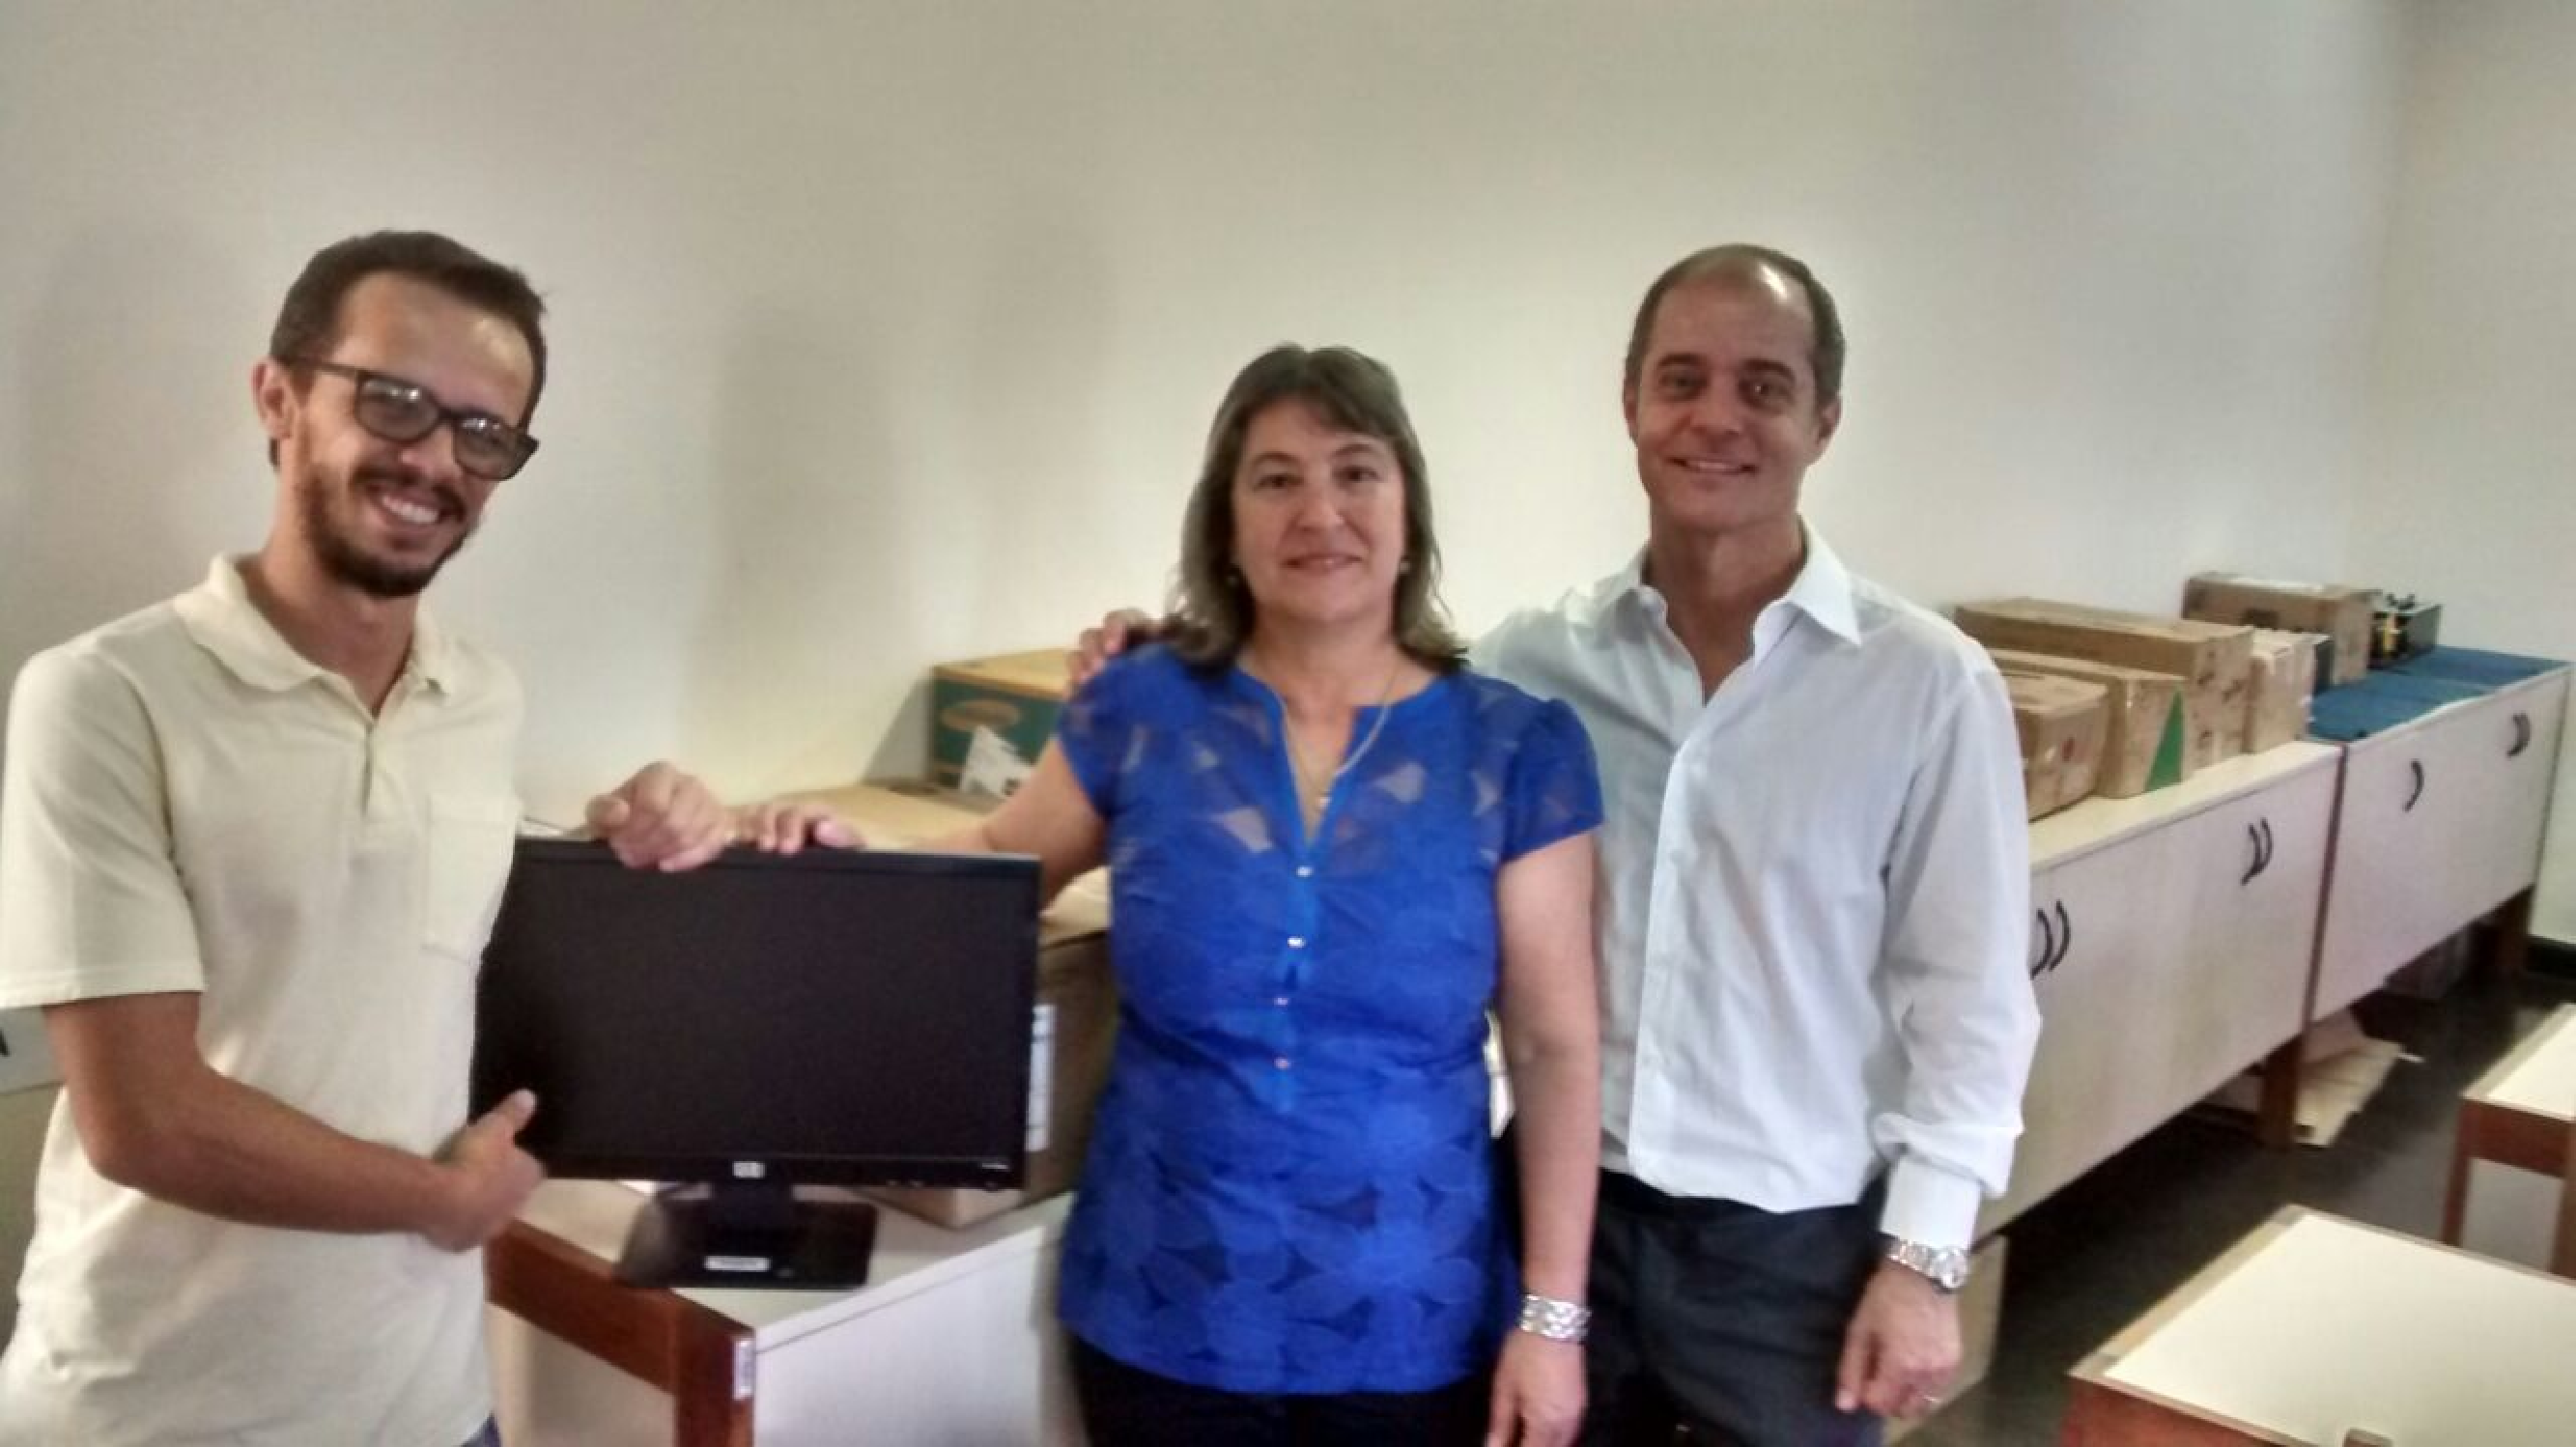
\includegraphics[scale=0.3]{figuras/cerimonia-de-entrega.pdf}
	\caption{Cerimônia de entrega de computadores em uma das instituições beneficiadas.}  \label{fig:entrega} 
\end{figure}

Na ocasião, o reitor da Universidade ressaltou a importância de programas que evidenciam a atuação do servidor público e, especialmente, dos professores em seu papel verdadeiro, o de servirem à sociedade.

Vale ressaltar que a entrega de computadores envolveu simultaneamente todos os projetos vinculados ao programa Reciclagem Digital, e por isso, movimentou os professores e alunos envolvidos.


\section{Resultados do ``Hospital da Máquinas''}

O projeto ``Hospital das Máquinas'' beneficiou instituições como a Escola Estadual Dom Benevides e Escola Estadual Dom Silvério, ambas localizadas na cidade Mariana, com a manutenção e assistência de 37 computadores, sendo 22 na primeira escola citada e 15 na segunda escola citada.

O bolsista Brian formatou o laboratório dessas duas escolas instalando o sistema operacional livre Linux Mint 17.3 conforme Figuras \ref{fig:tela1} e \ref{fig:tela2}. Além disso, um pacote de programas e jogos educativos foram instalados em todos os computadores. 

\begin{figure}[H]
	\centering
	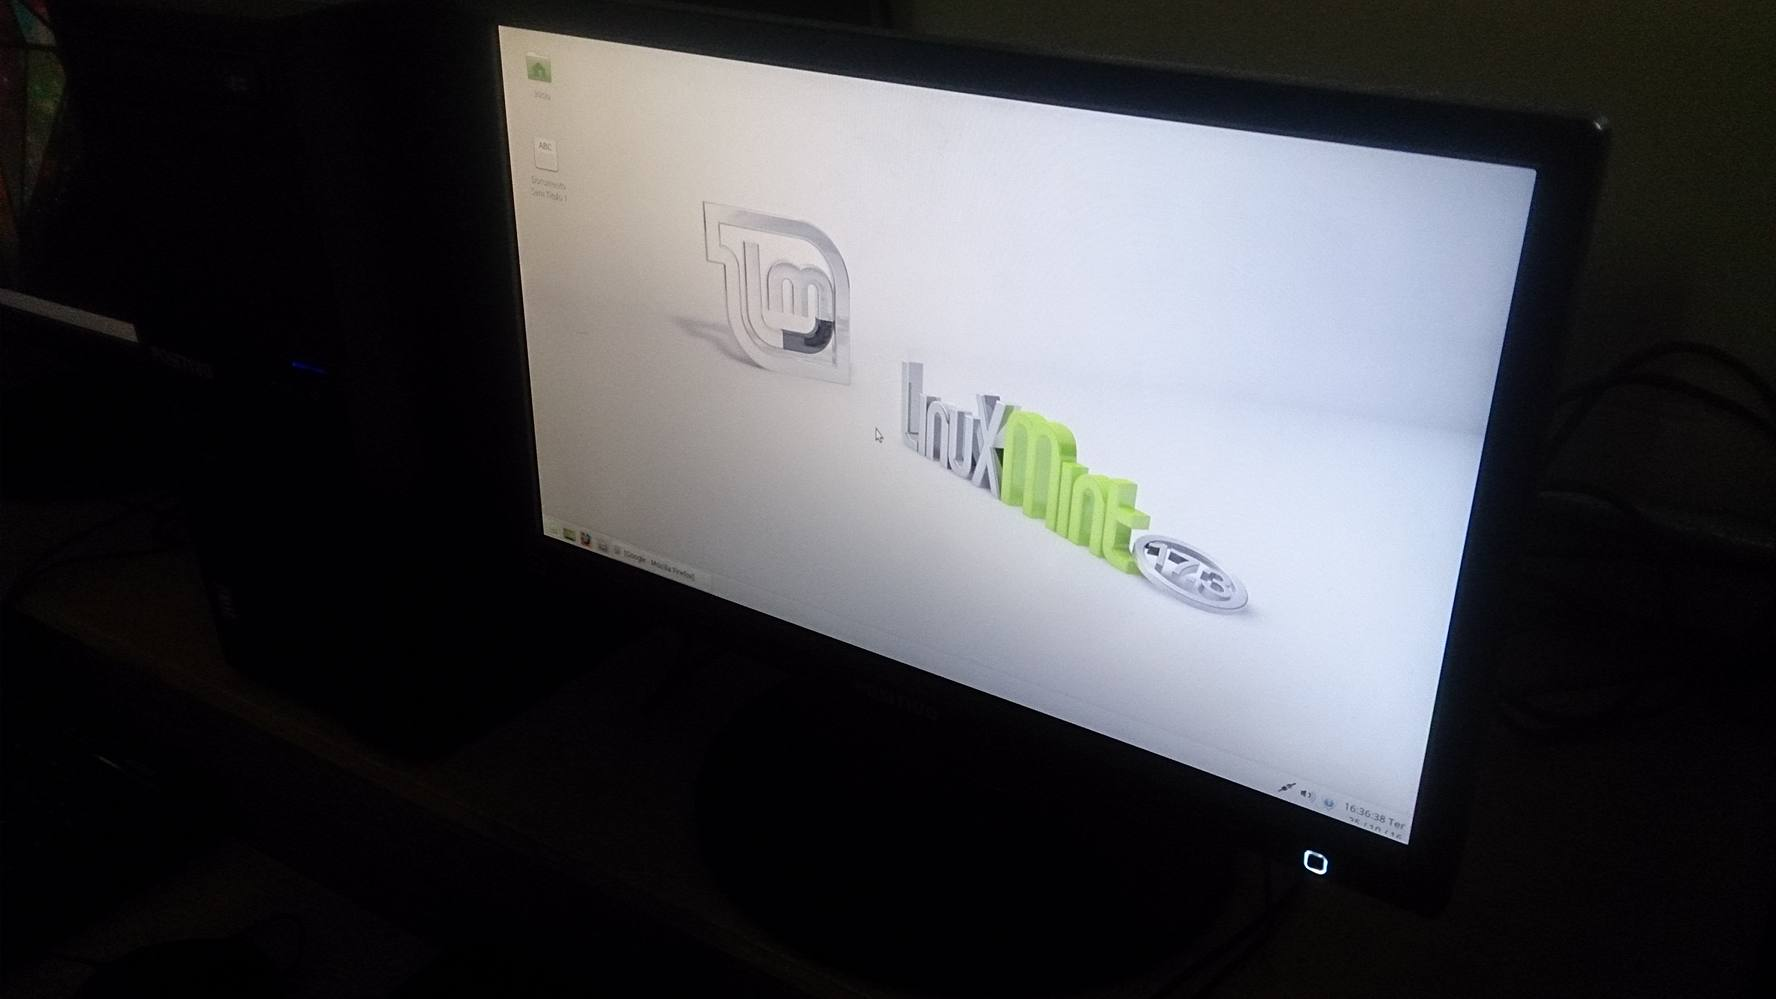
\includegraphics[scale=0.2]{figuras/cris01.jpg}
	\caption{Tela de um computador da Escola Estadual Dom Benevides.}
	\label{fig:tela1}
\end{figure}

\begin{figure}[H]
	\centering
	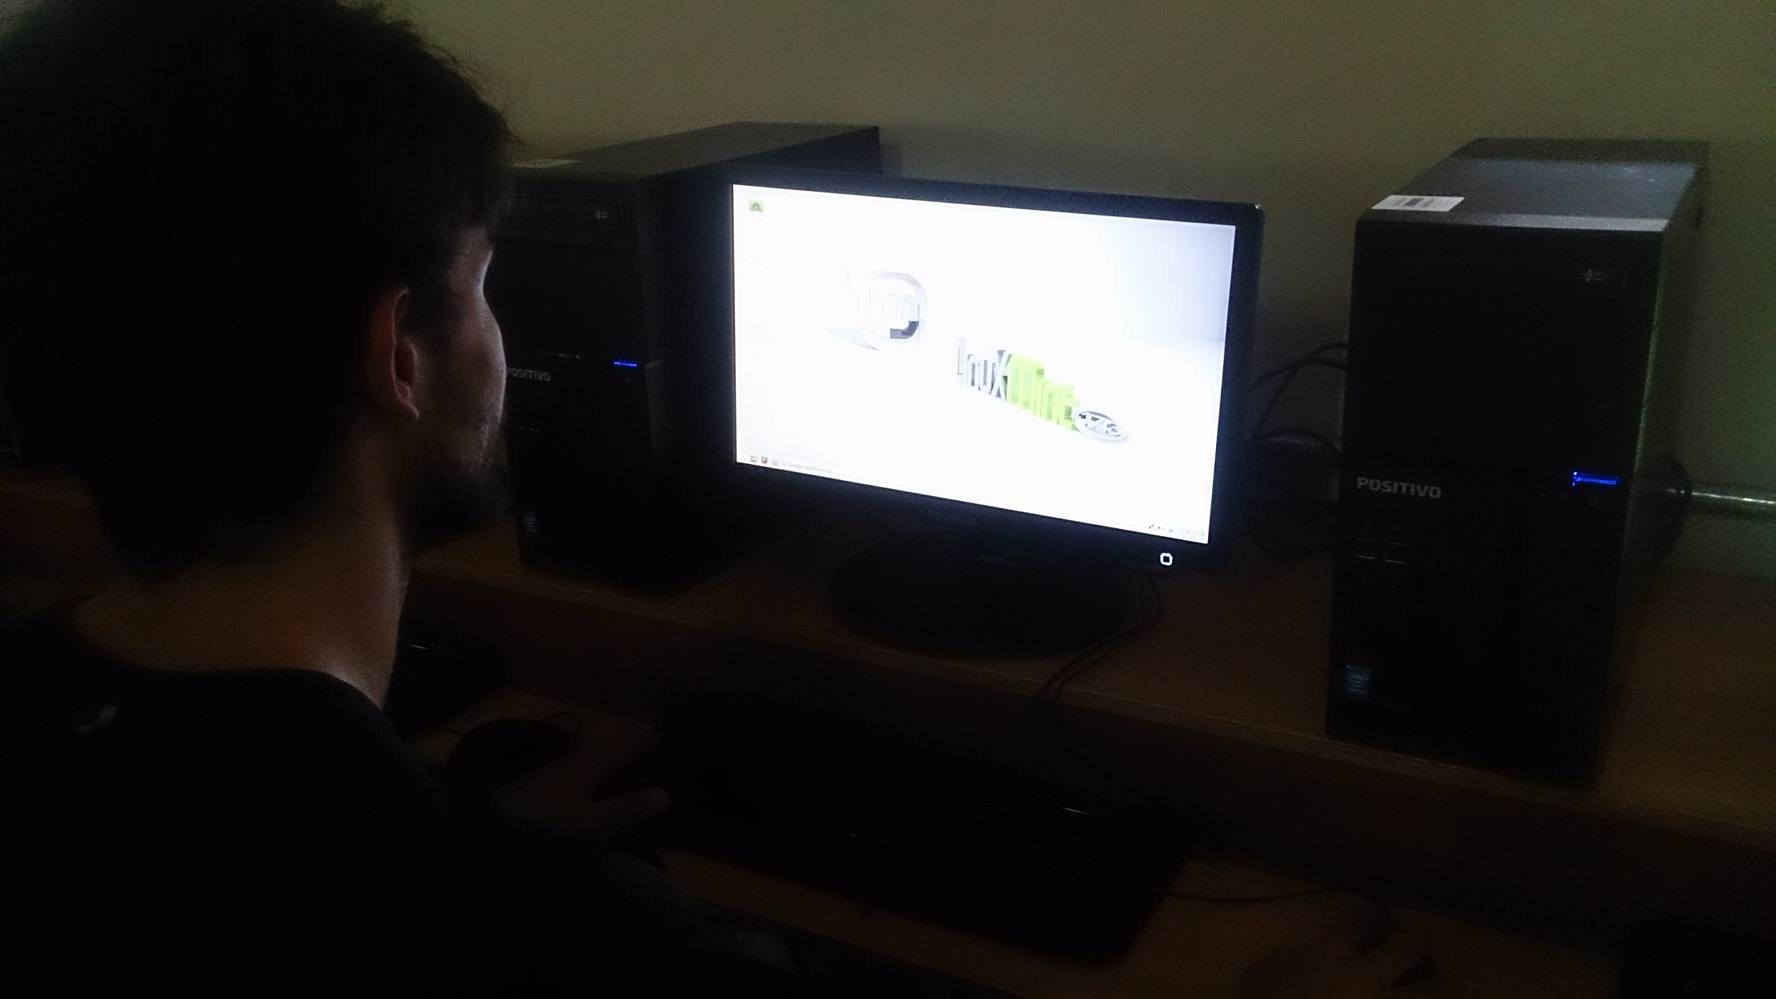
\includegraphics[scale=0.2]{figuras/cris02.jpg}
	\caption{Bolsista Brian trabalhando em um computador na Escola Estadual Dom Benevides.}
	\label{fig:tela2}
\end{figure}

Na Figura \ref{fig:tela3} é possível verificar alguns computadores que foram formatados no laboratório da Escola Estadual Dom Benevides.

\begin{figure}[H]
	\centering
	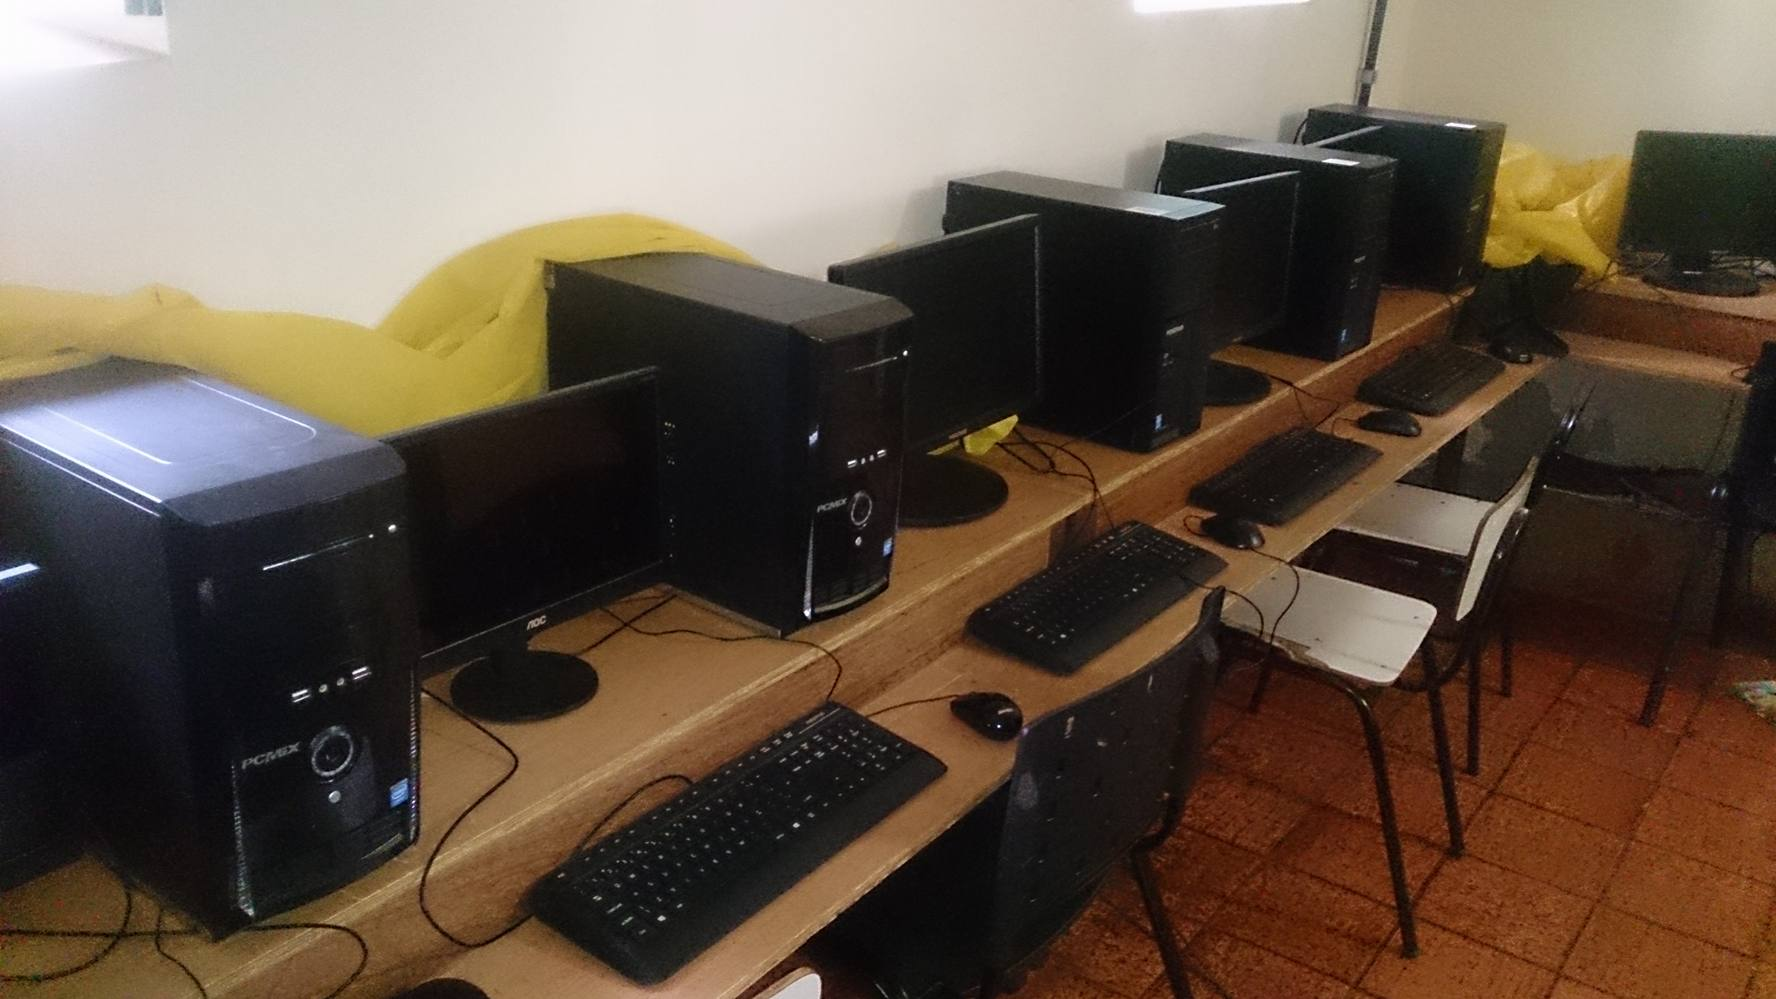
\includegraphics[scale=0.2]{figuras/cris03.jpg}
	\caption{Laboratório trabalhado da Escola Estadual Dom Benevides.}
	\label{fig:tela3}
\end{figure}

A Figura \ref{fig:tela4} mostra o bolsista Brian recebendo a assinatura no comprovante de realização de atividades (Figura \ref{fig:tela9}) de execução do serviço da responsável pela Escola Estadual Dom Benevides.

\begin{figure}[H]
	\centering
	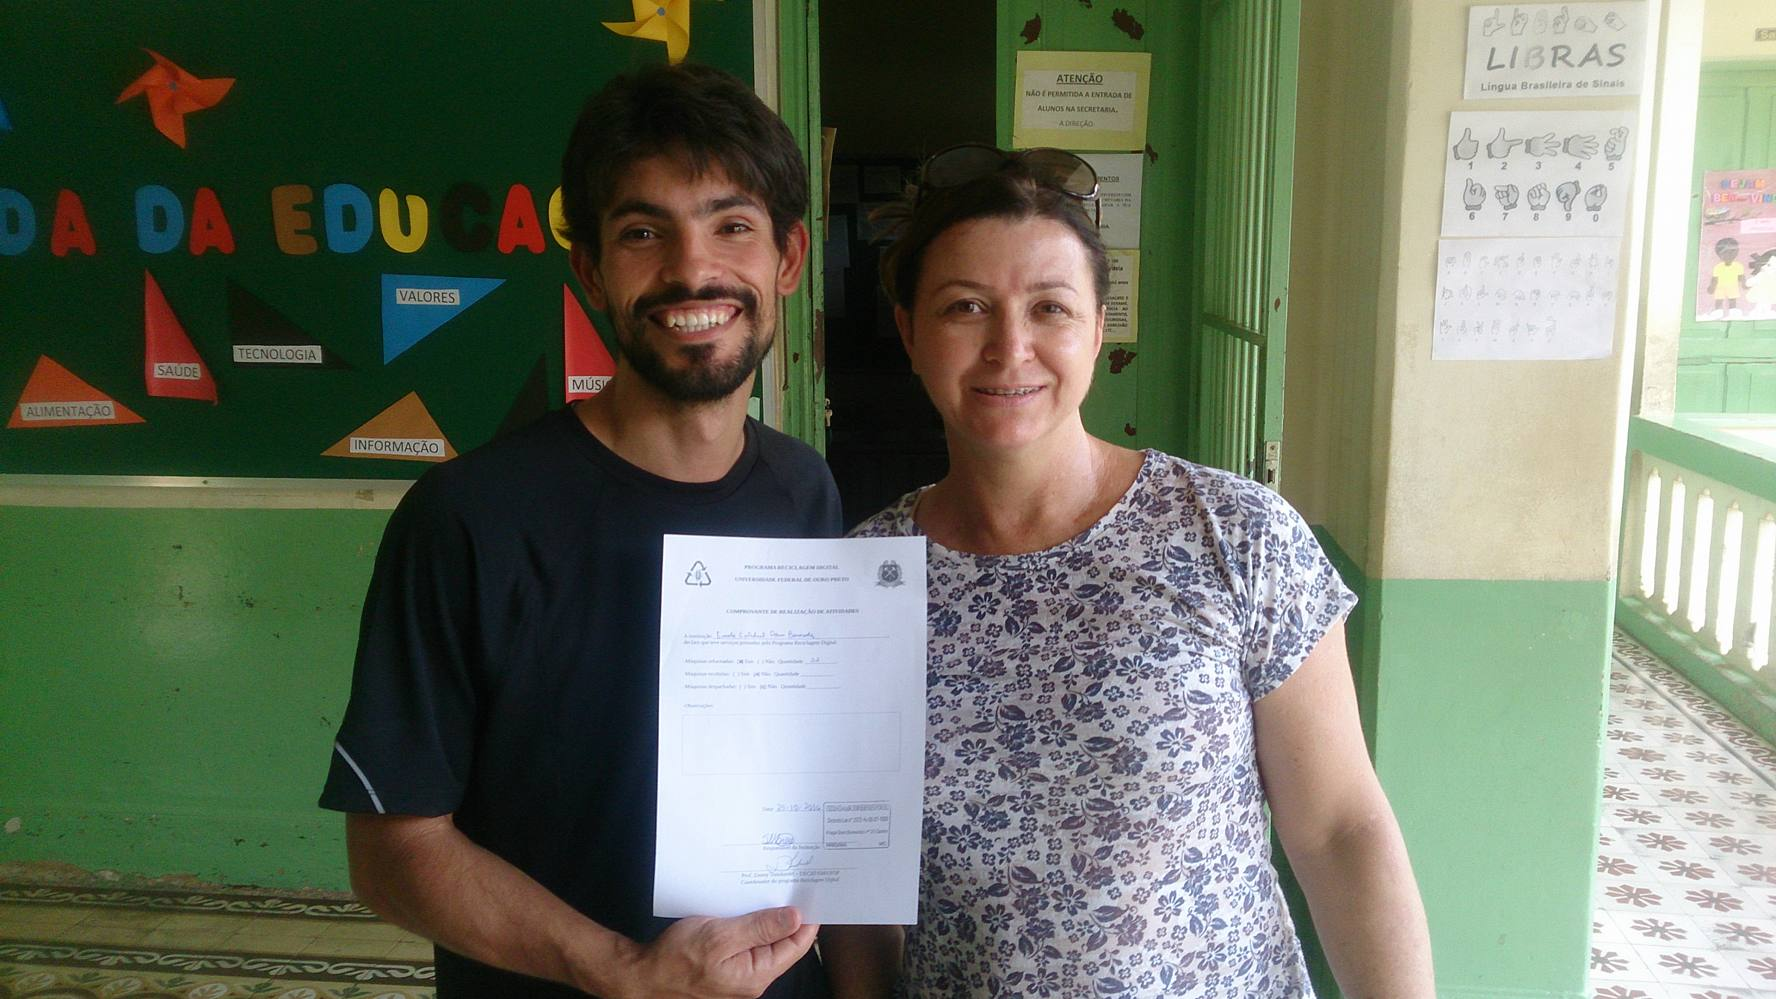
\includegraphics[scale=0.2]{figuras/cris04.jpg}
	\caption{Assinatura da responsável pela Escola Estadual Dom Benevides.}
	\label{fig:tela4}
\end{figure}

\begin{figure}[H]
	\centering
	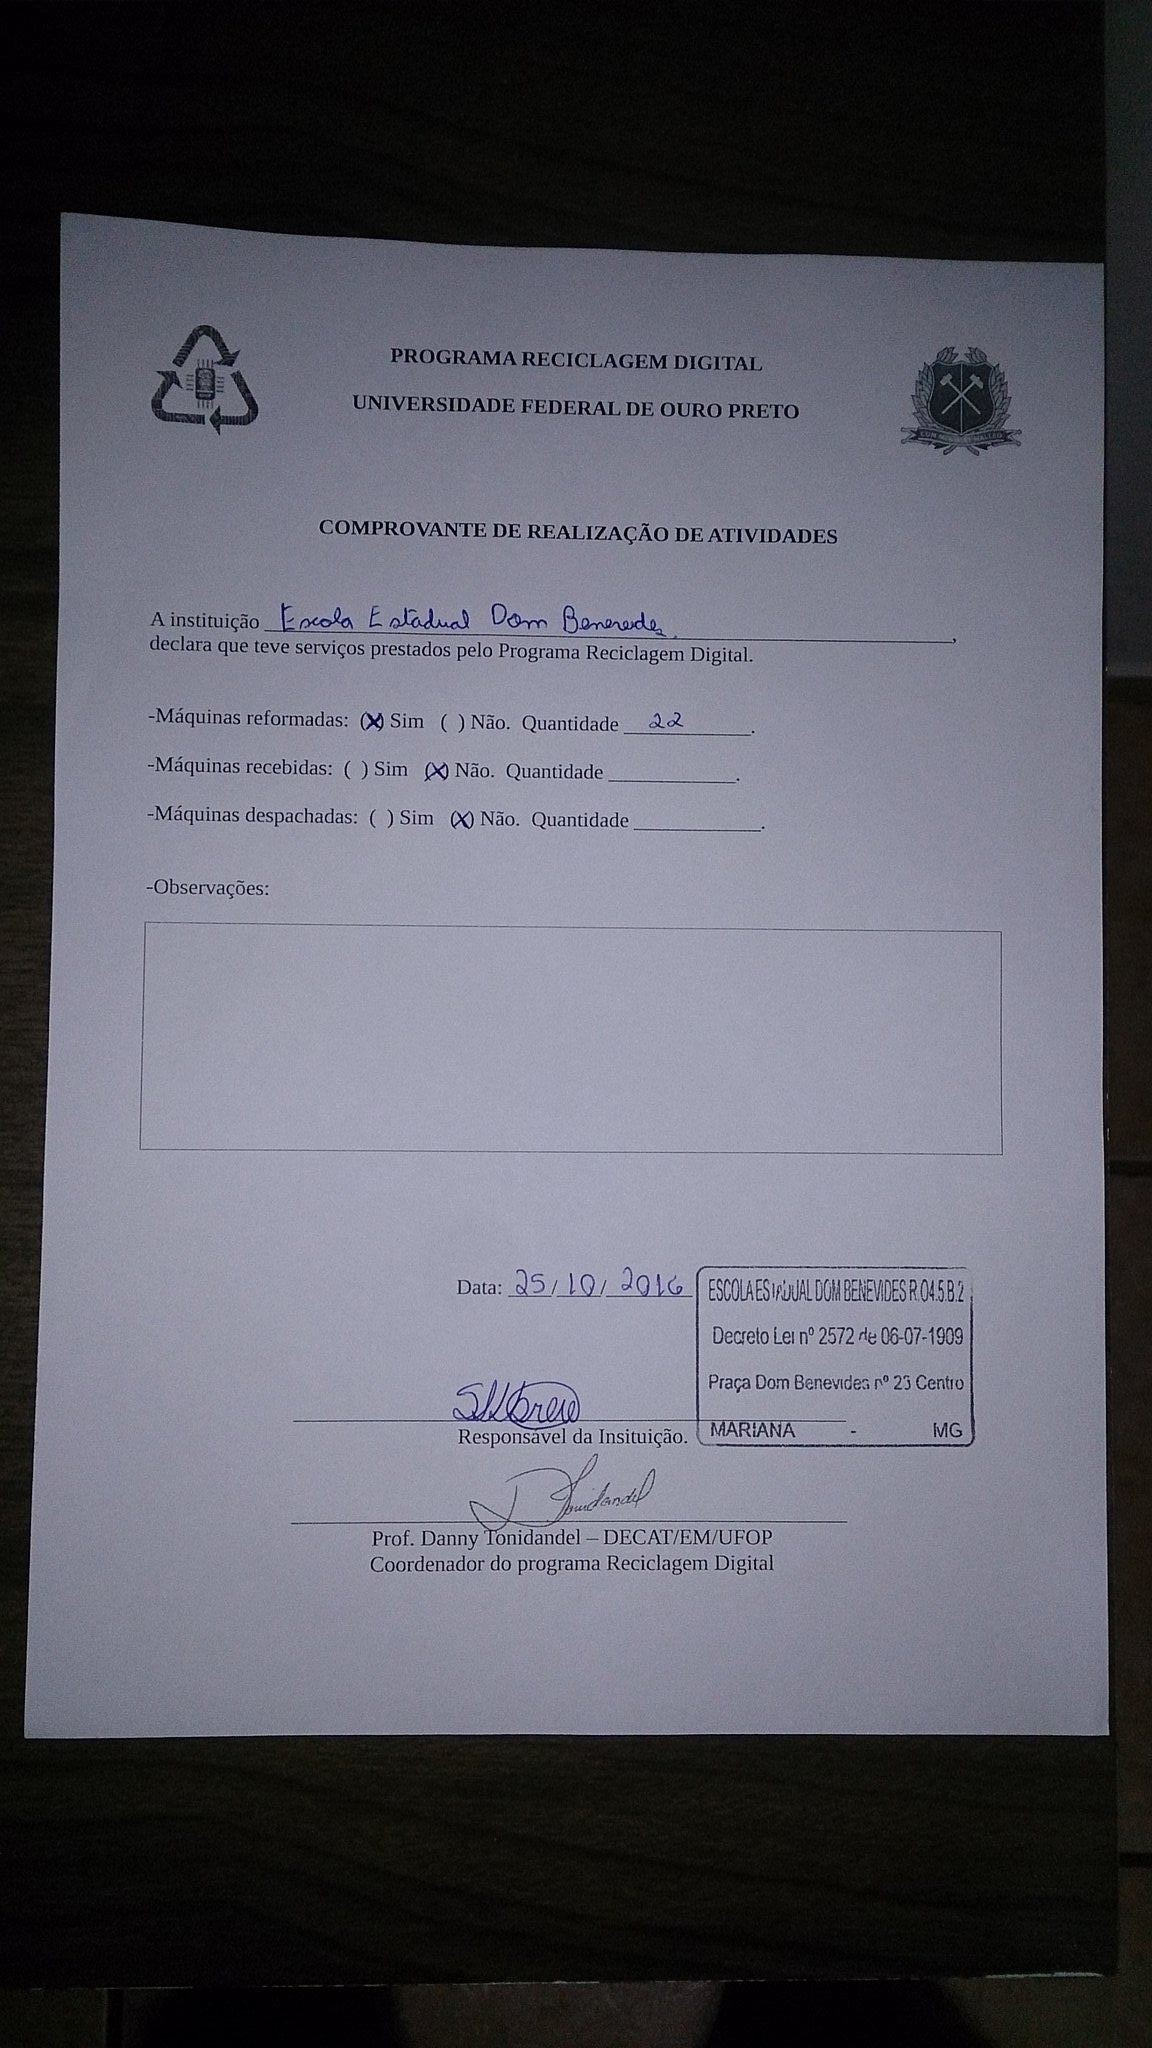
\includegraphics[scale=0.3]{figuras/cris09.jpg}
	\caption{Comprovante de realização de atividades na Escola Estadual Dom Benevides.}
	\label{fig:tela9}
\end{figure}

A Figura \ref{fig:tela5} mostra a impactante imagem do laboratório da Escola Estadual Dom Silvério, antes do trabalho do programa ``Hospital das Máquinas'' acontecer. Observe-se que ele estava totalmente inutilizado por falta de manutenção e reparos. A Figura \ref{fig:tela6}, por sua vez, ilustra como ficou o laboratório após o trabalho.

\begin{figure}[H]
	\centering
	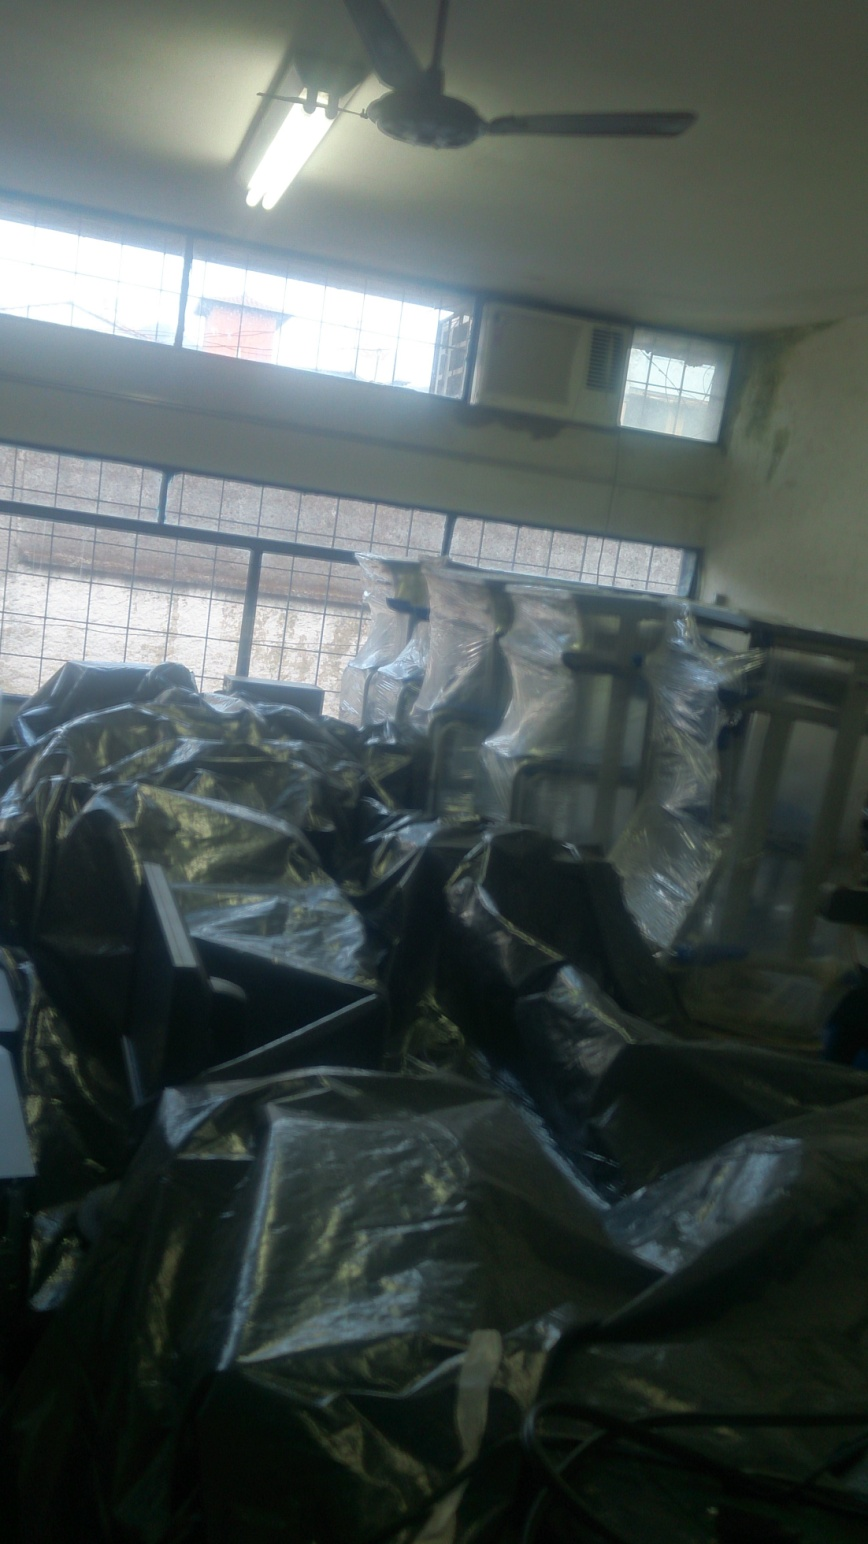
\includegraphics[scale=0.6]{figuras/cris05.jpg}
	\caption{Laboratório da Escola Estadual Dom Silvério antes do trabalho do programa ``Hospital das Máquinas''.}
	\label{fig:tela5}
\end{figure}

\begin{figure}[H]
	\centering
	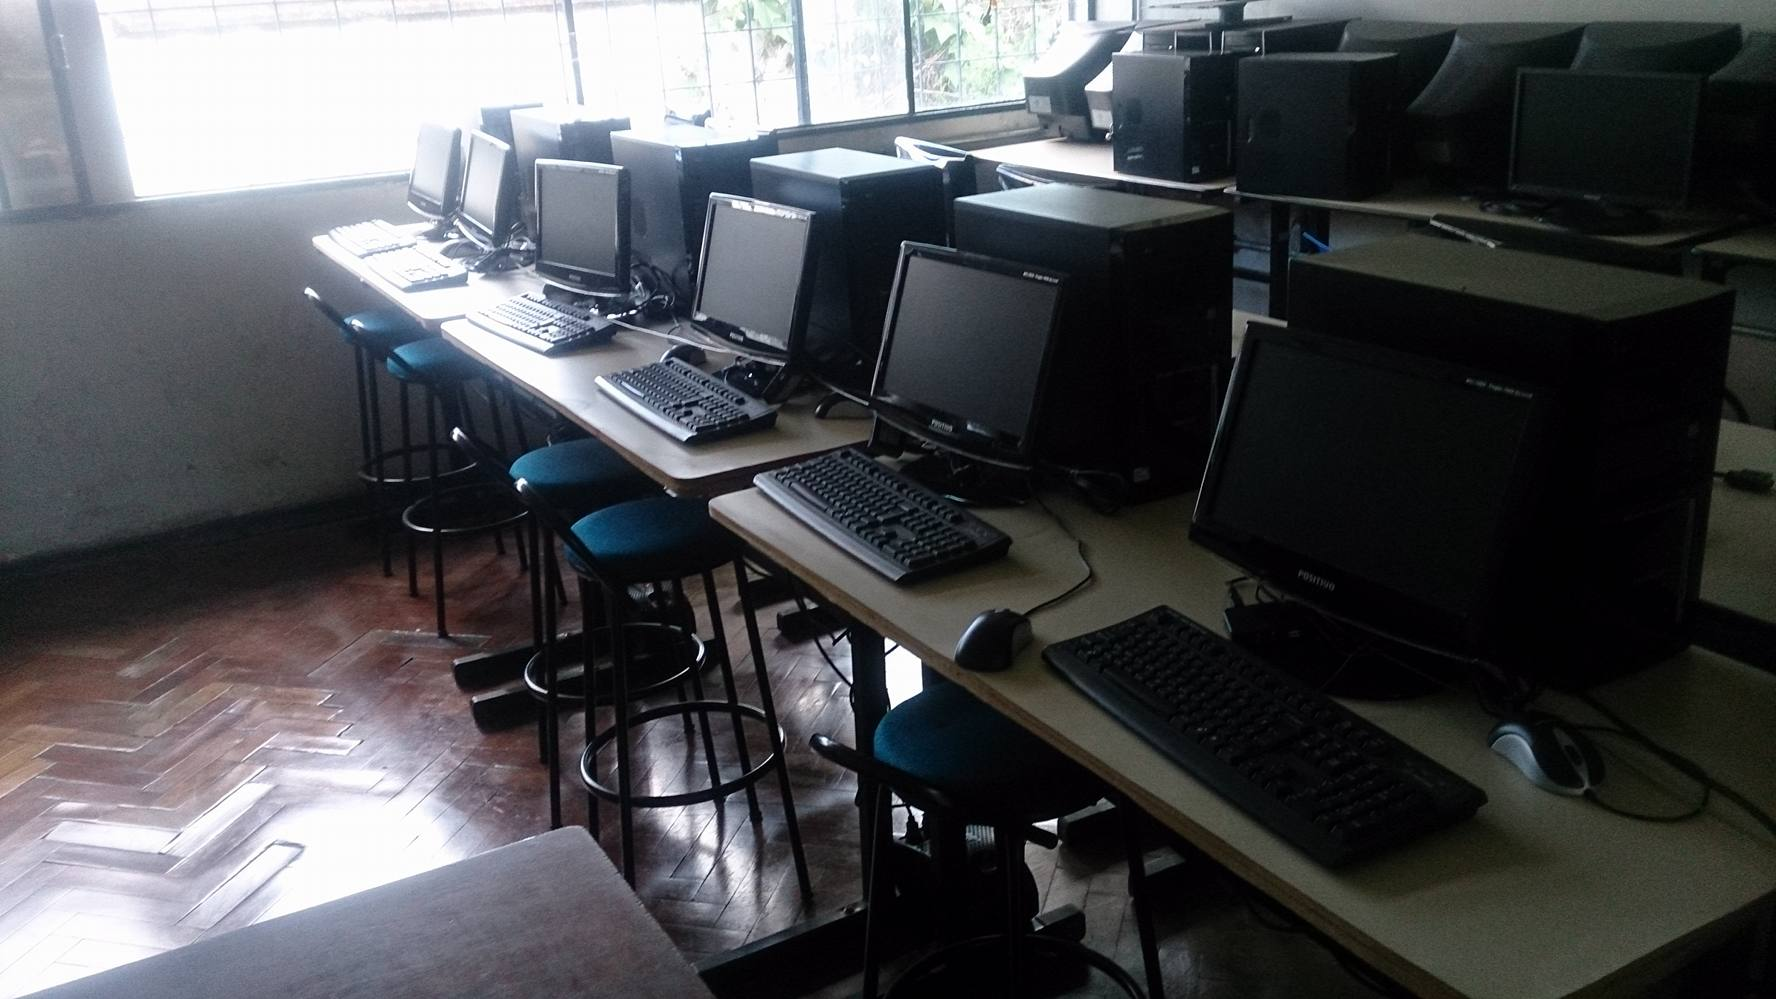
\includegraphics[scale=0.2]{figuras/cris06.jpg}
	\caption{Laboratório da Escola Estadual Dom Silvério depois do trabalho do programa ``Hospital das Máquinas''.}
	\label{fig:tela6}
\end{figure}

As Figuras \ref{fig:tela7}, \ref{fig:tela8} e \ref{fig:tela11} mostram o laboratório da Escola Estadual Dom Silvério sendo testado pelos bolsistas Aluizio e Brian.

\begin{figure}[H]
	\centering
	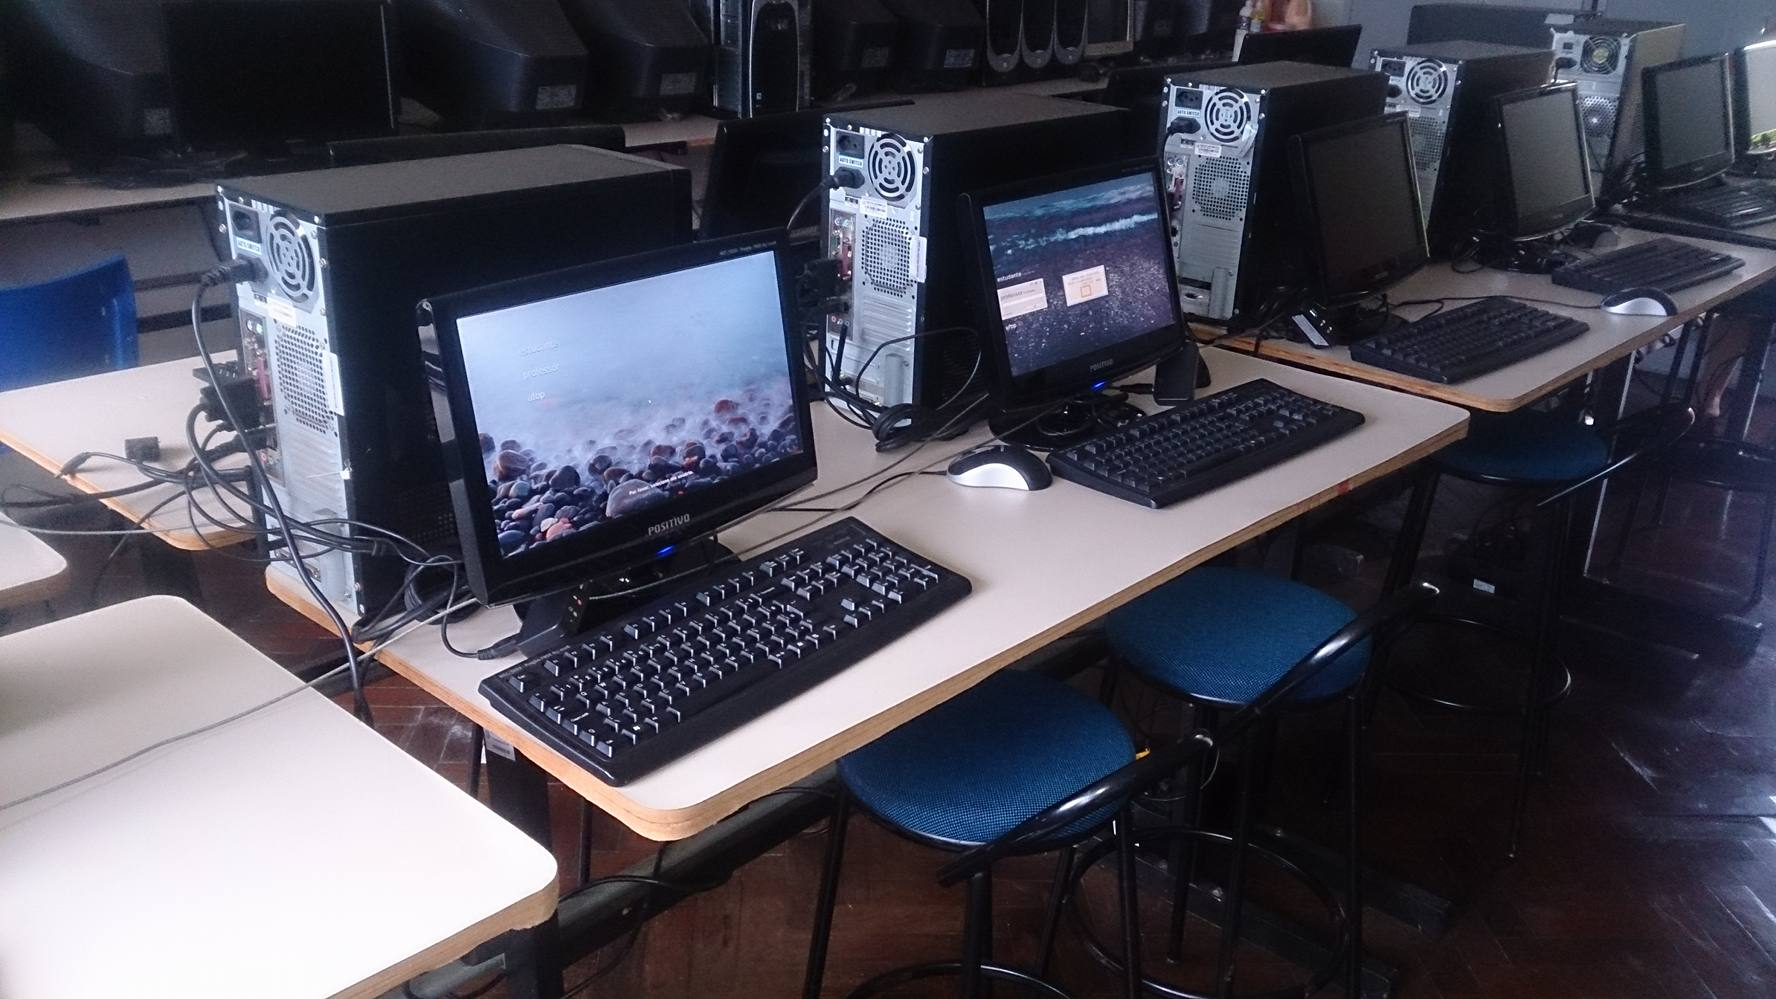
\includegraphics[scale=0.2]{figuras/cris07.jpg}
	\caption{Teste do laboratório da Escola Estadual Dom Silvério.}
	\label{fig:tela7}
\end{figure}

\begin{figure}[H]
	\centering
	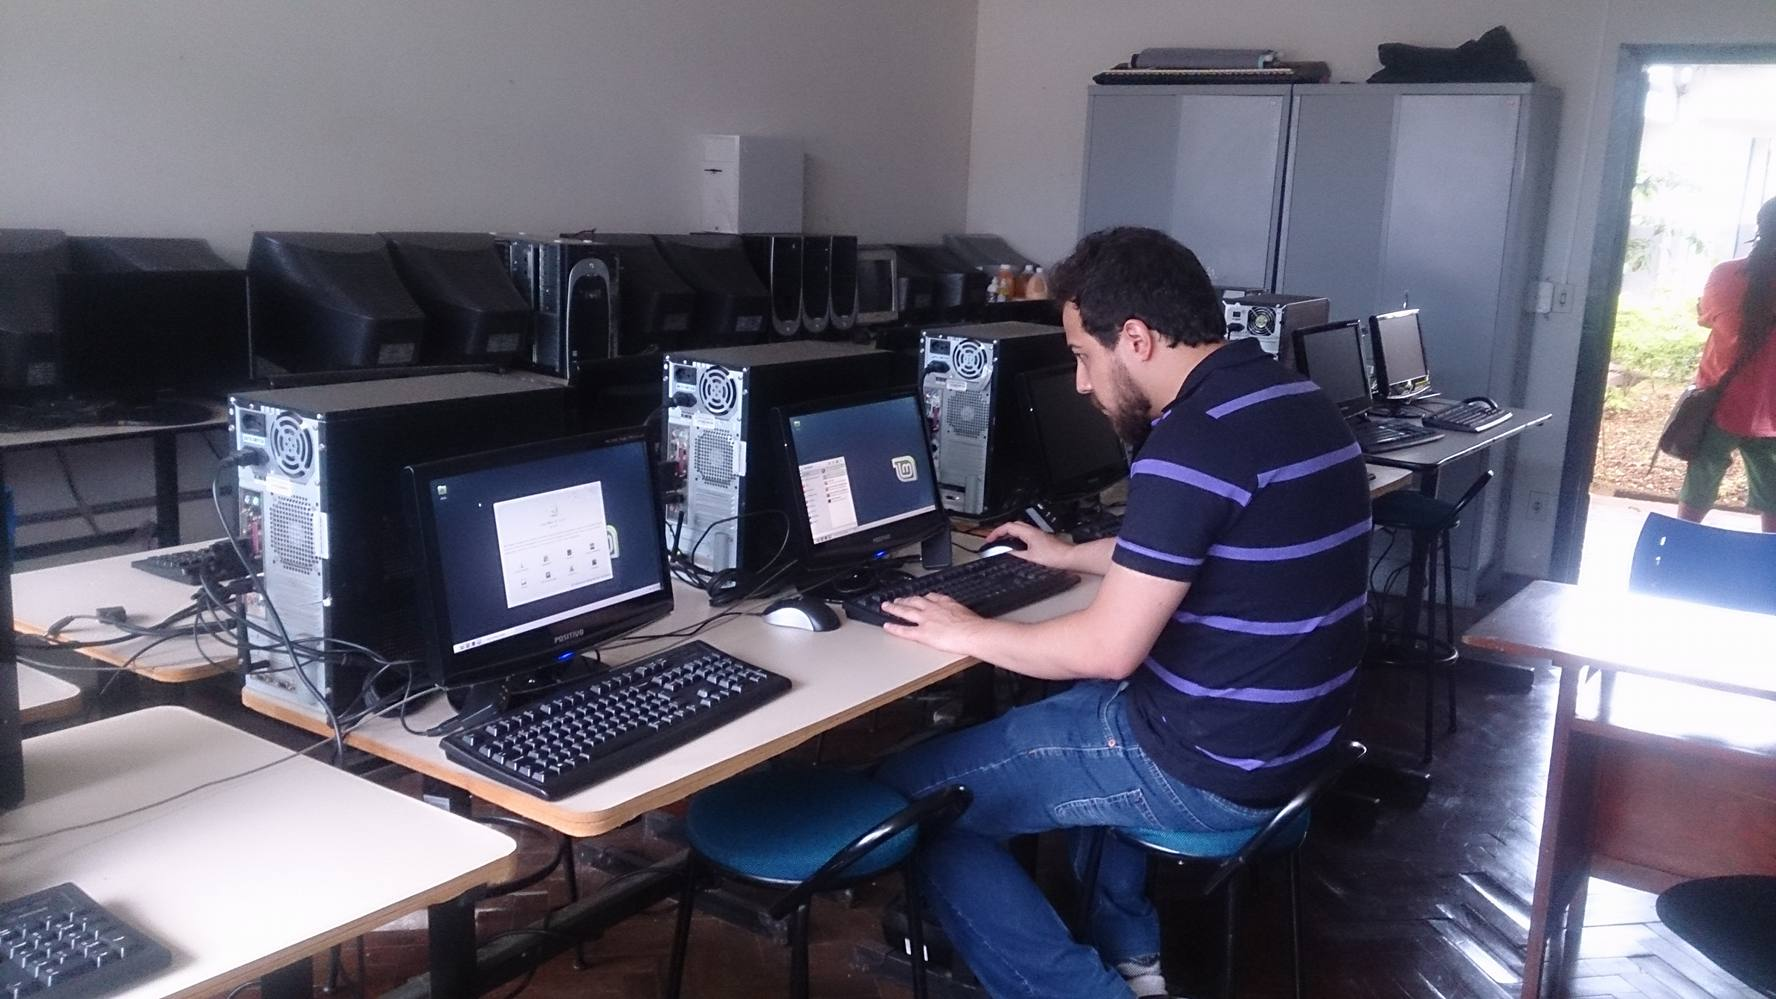
\includegraphics[scale=0.2]{figuras/cris08.jpg}
	\caption{Teste do laboratório da Escola Estadual Dom Silvério pelo bolsista Aluizio.}
	\label{fig:tela8}
\end{figure}

\begin{figure}[H]
	\centering
	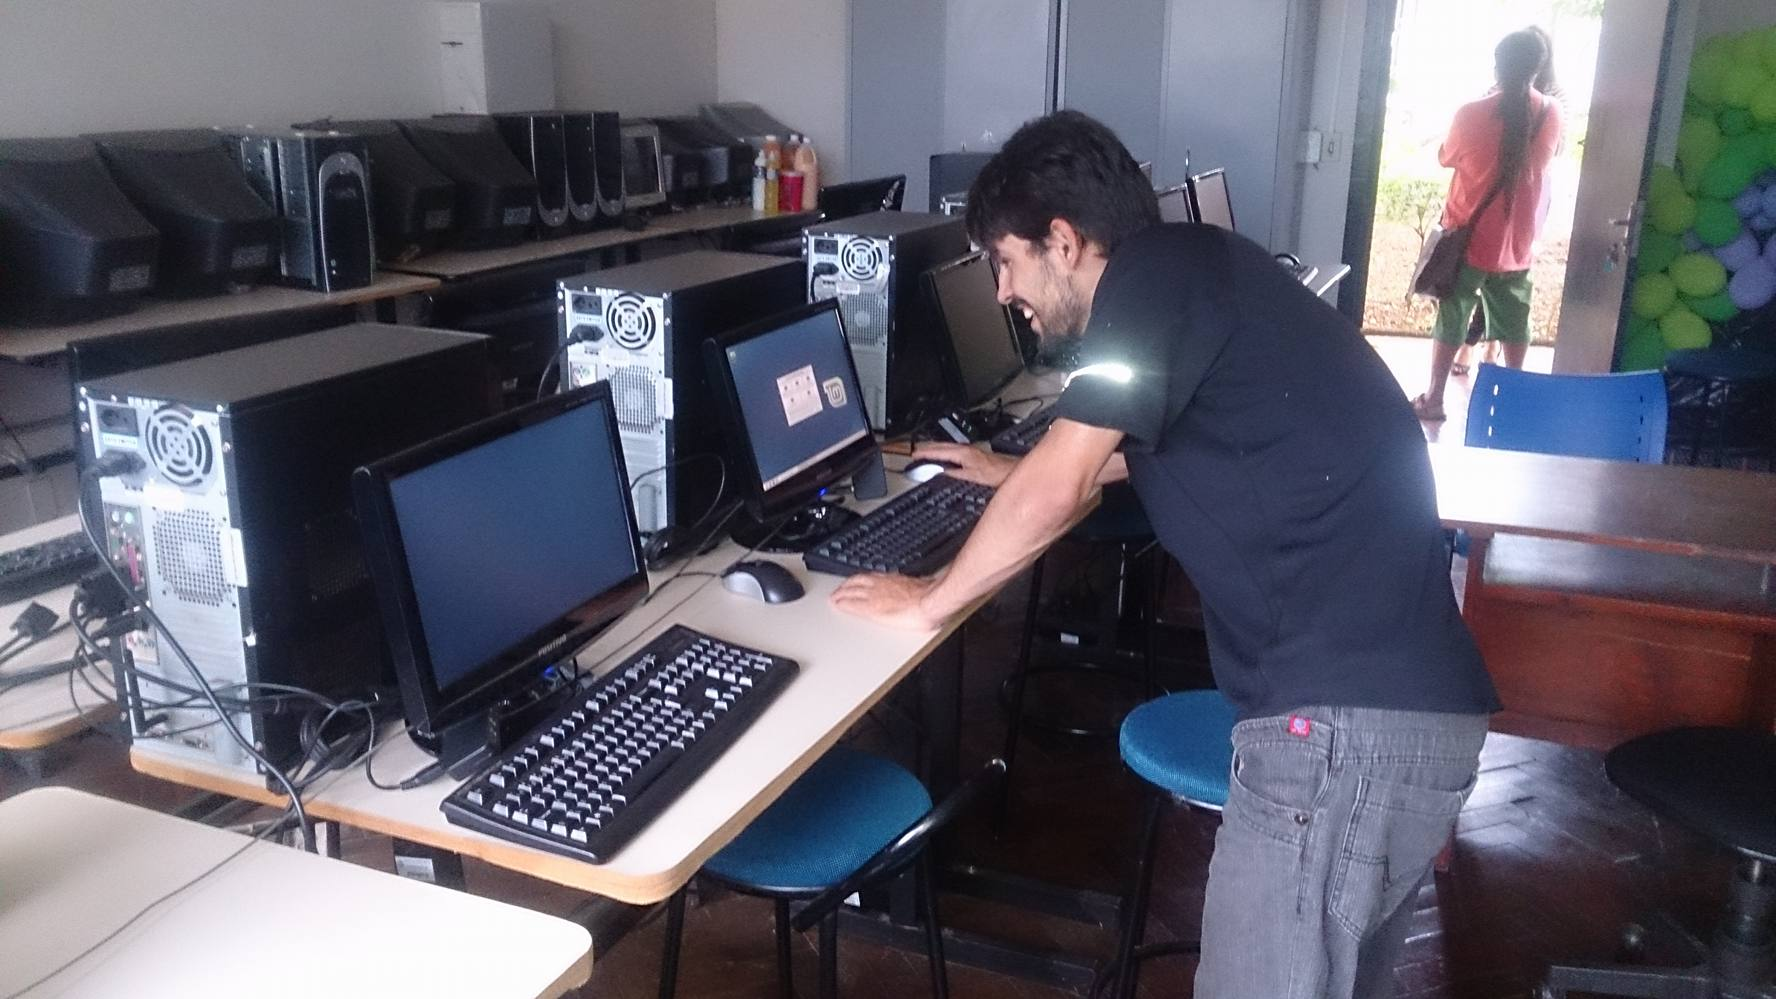
\includegraphics[scale=0.2]{figuras/cris11.jpg}
	\caption{Teste do laboratório da Escola Estadual Dom Silvério pelo bolsista Brian.}
	\label{fig:tela11}
\end{figure}

A Figura \ref{fig:tela10} mostra a assinatura no comprovante de realização de atividades de execução do serviço pela Escola Estadual Dom Silvério.

\begin{figure}[H]
	\centering
	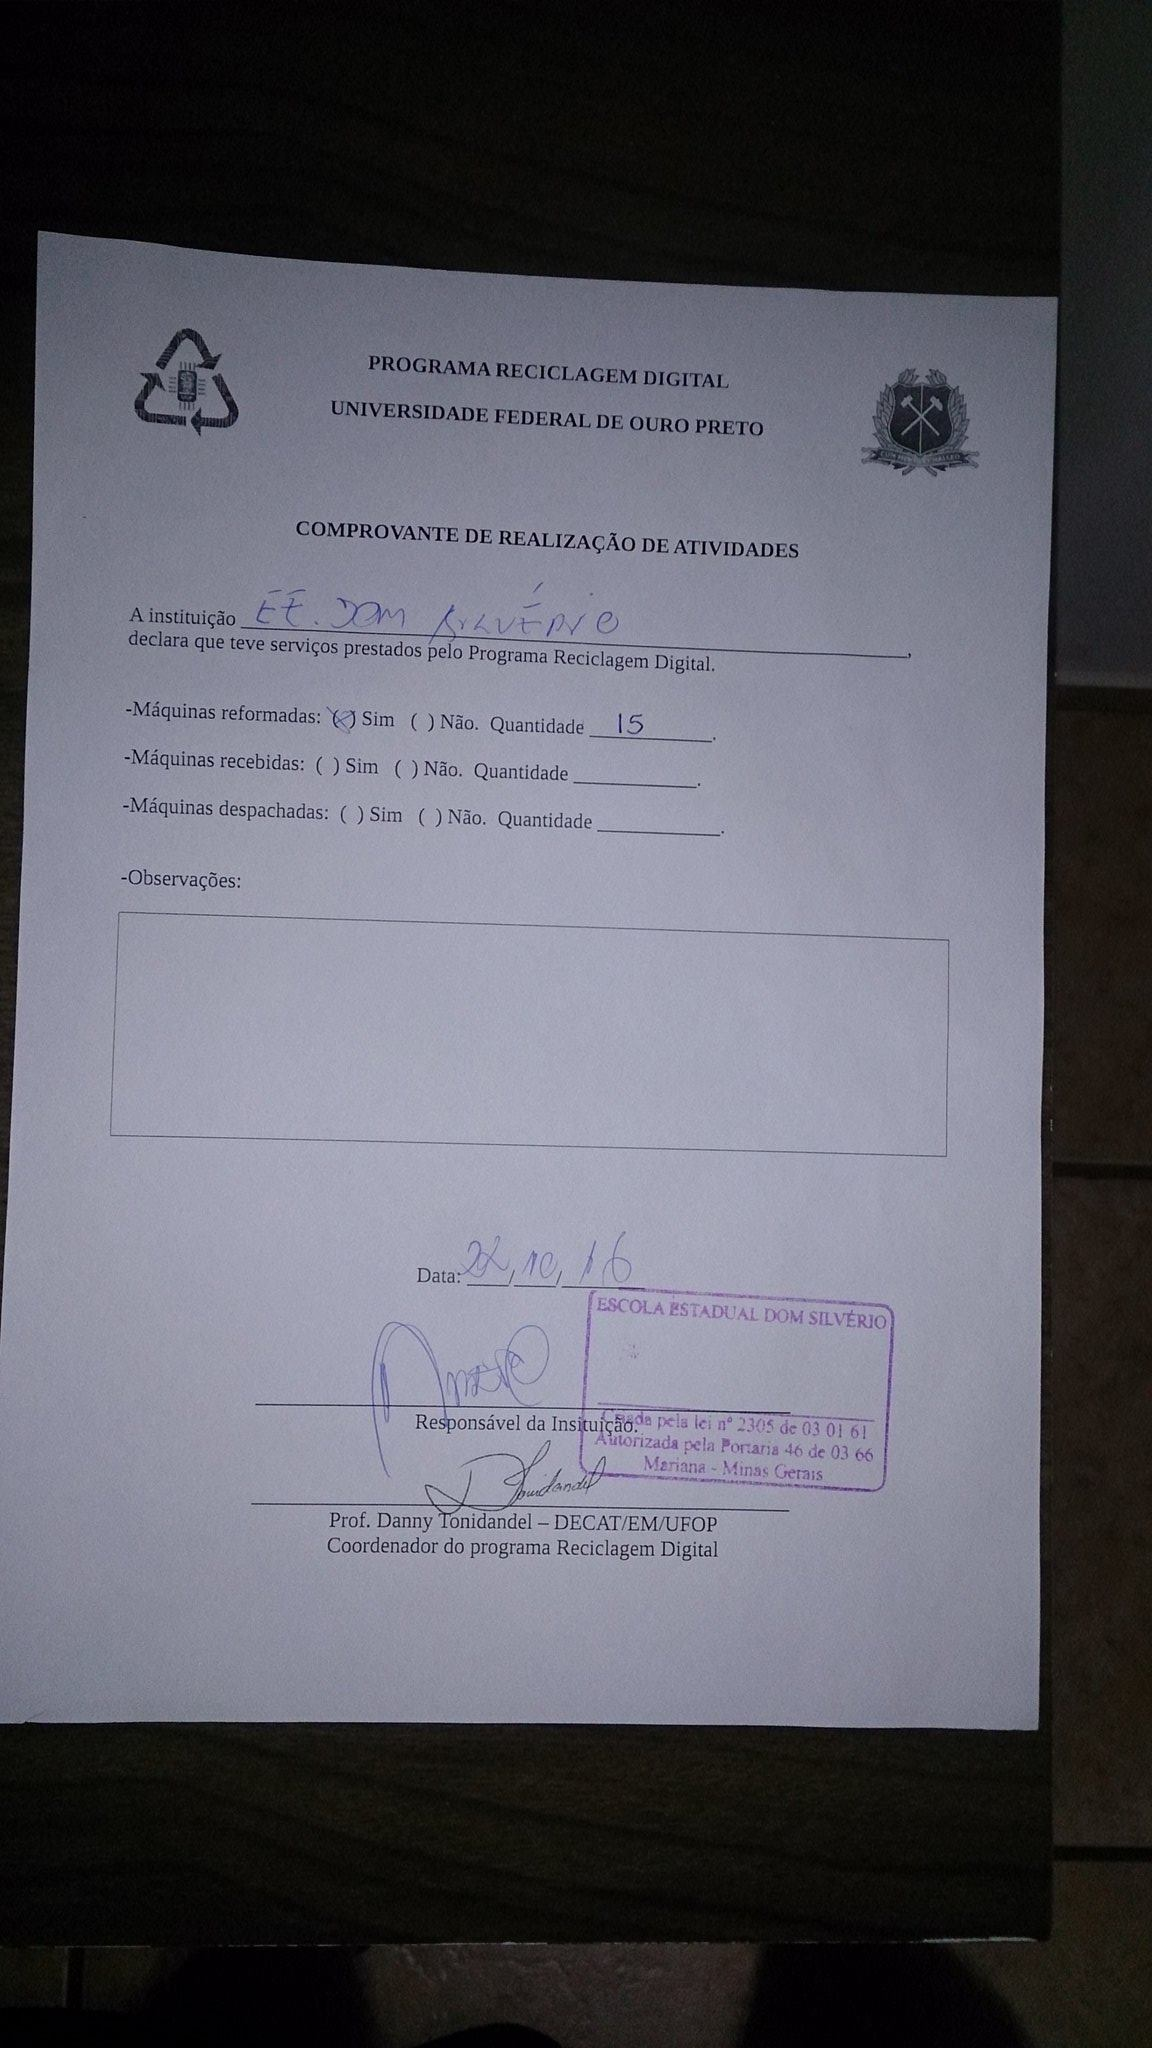
\includegraphics[scale=0.2]{figuras/cris10.jpg}
	\caption{Comprovante de realização de atividades na Escola Estadual Dom Silvério.}
	\label{fig:tela10}
\end{figure}

\section{Resultados do ``Manufatura Reversa''}

A engenharia reversa possibilitou a aquisição de componentes e peças
que foram úteis no desenvolvimento de alguns projetos de pesquisa na UFOP, como o projeto do professor Helder Luis, do DEARQ, que necessitava de material para a \textbf{construção de um forno à gás automático}, em um  trabalho de conclusão de curso realizado por um aluno do curso de Engenharia de Controle e Automação, como parte de uma pesquisa desenvolvida pelo departamento de Arquitetura e Urbanismo.

Outra articulação com a pesquisa que gerou bons resultados, e que podemos ressaltar, foi o \textbf{desenvolvimento de uma solda de termopares por descarga capacitiva} (figura \ref{fig:solda}), a partir de uma solicitação do professor responsável peço laboratório de usinagem, prof. Igor Pereira. Este, dentre todas as solicitações ao projeto, foi a que demandou maior esforço de estudo e planejamento por parte do aluno, envolvendo a área de eletrônica analógica, confecção de placas de circuito impresso, além de propiciar ao estudante o aprofundamento na física inerente ao processo de soldagem, área que não faz parte (diretamente) do escopo da Engenharia de Controle e Automação.

O projeto ``obrigou'' o estudante a desenvolver modelos de simulação de circuitos, já que o modelo passado pelo prof. da Engenharia Mecânica era baseado em um vídeo da Internet, que não possuía nenhuma garantia de funcionamento (e, por diversas vezes, não funcionava como deveria).

\begin{figure}[H]
	\centering
	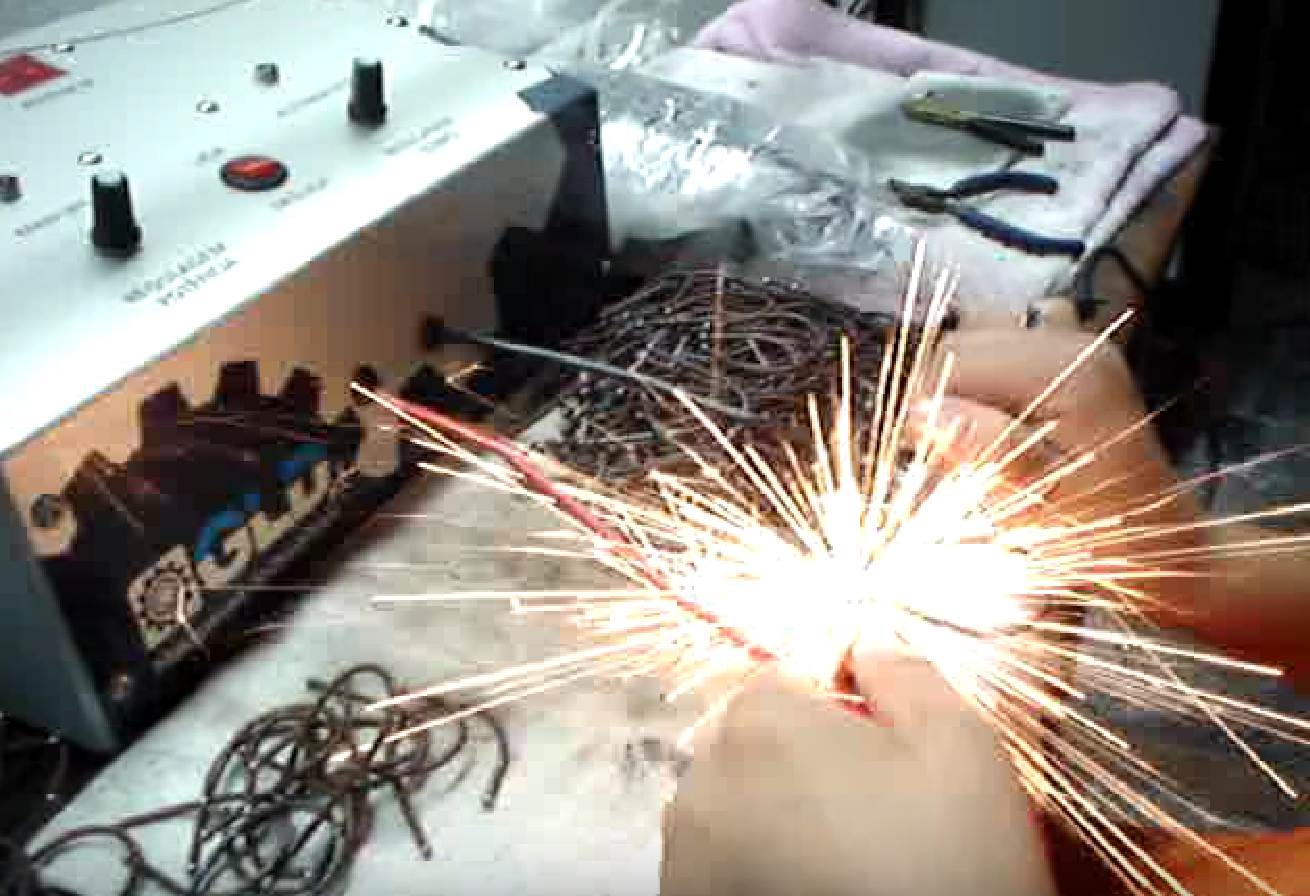
\includegraphics[scale=0.7]{figuras/solda-capacitiva.pdf}
	\caption{Solda por descargha capacitiva para o laboratório de usinagem (imagem ilustrativa).}  \label{fig:solda} 
\end{figure}

O equipamento consiste em um banco de capacitores ligados em paralelo que, quando ligados a uma carga, descarrega toda a energia carregada em forma de corrente elétrica, fundindo por resistência a carga a outro material metálico. A tensão aplicada na carga é igual a soma das tensões aplicadas em cada capacitor. Todos os capacitores são alimentados com a mesma fonte.

O primeiro trabalho do aluno foi se familiarizar com a teoria por trás do conceito de solda capacitiva, além da simulação de circuitos eletrônicos (figura \ref{fig:simulacao1}) e a confecção dos mesmos, especialmente por se tratar de estudante dos primeiros períodos da graduação em Engenharia de Controle e Automação.

\begin{figure}[H]
	\centering
	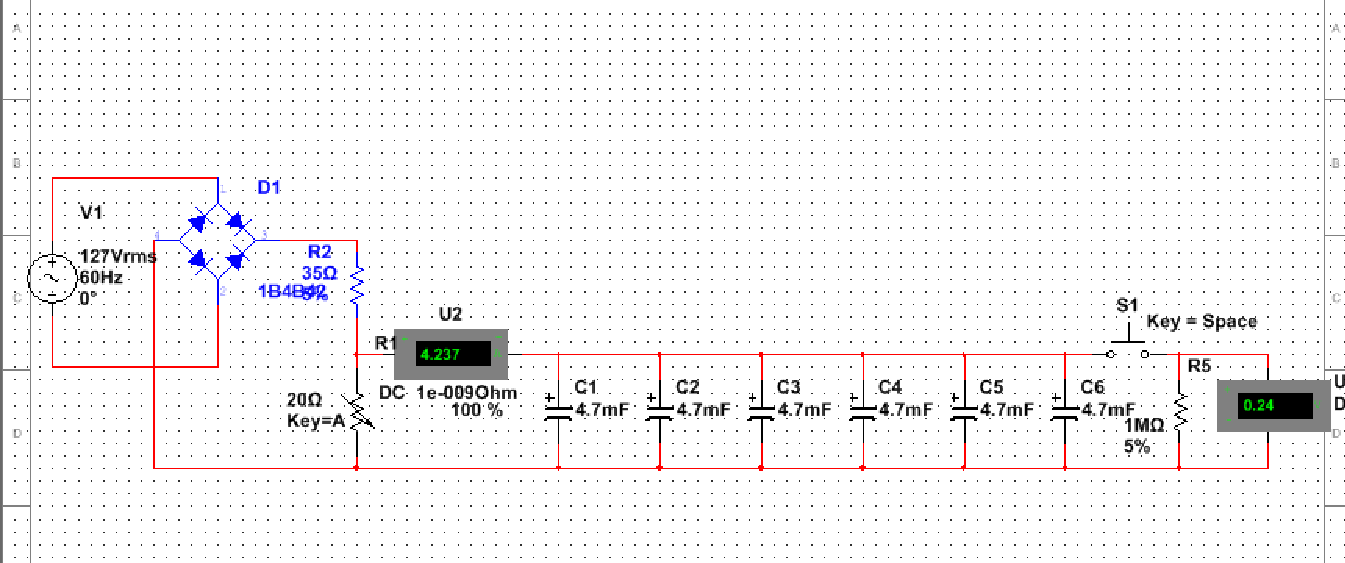
\includegraphics[scale=0.7]{figuras/simulacao1.pdf}
	\caption{Simulação da por descarga capacitiva no software proteus.}  \label{fig:simulacao1} 
\end{figure}

O desafio era, portanto, utilizarmos de material reciclado e retirado, em maior parte, do setor de desfazimento da UFOP. Isto aconteceu após a saída do bolsista Gabriel (estudante de Engenharia Mecânica) do referido projeto e a entrada (no último mês) do aluno Heitor Novais (estudante de Engenharia de Controle e Automação). 

Adequando-se à ideia central do projeto, o protótipo da solda capacitiva pode ser adaptado a materiais reciclados a partir do lixo eletrônico.
Capacitores podem ser encontrados em placas-mãe, oriundas de computadores de mesa, conforme ilustra a figura \ref{fig:capacitores}.

\begin{figure}[H]
	\centering
	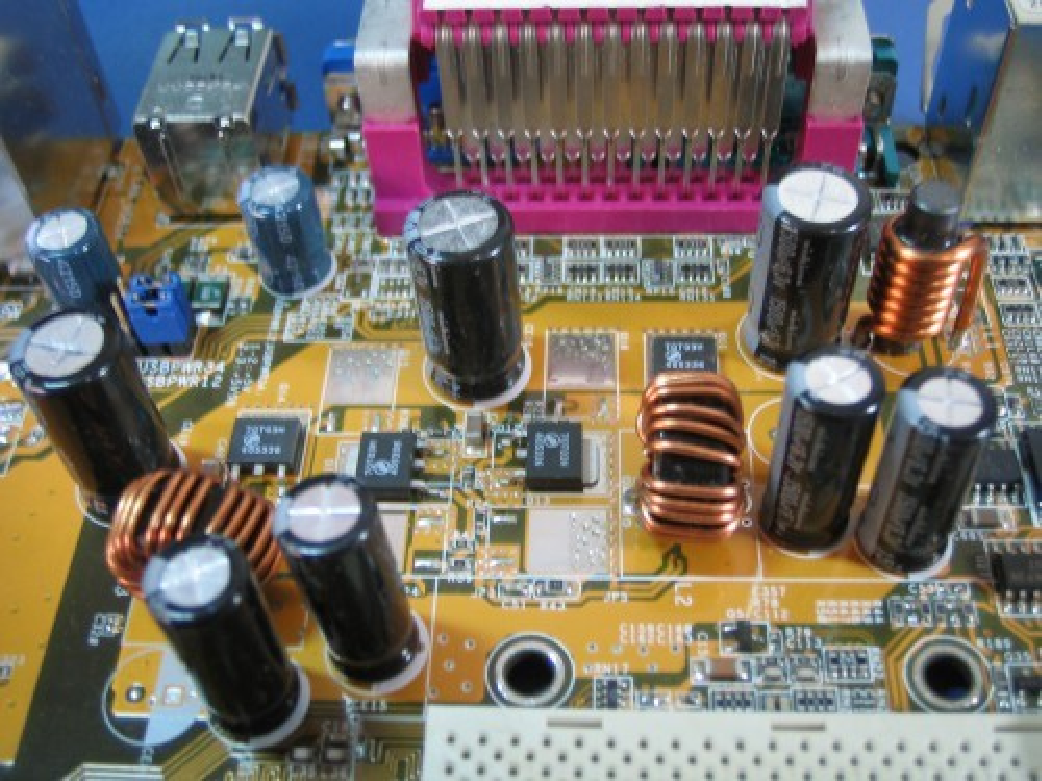
\includegraphics[scale=0.7]{figuras/capacitores.pdf}
	\caption{Capacitores podem ser encontrados em placas-mãe de computadores descartados.}  \label{fig:capacitores} 
\end{figure}

No equipamento em questão foram utilizados seis capacitores de $4700 \mu F$ e $50V$, todos eles ligados em paralelo. Para isso, a tensão da fonte, que foi substituída por uma fonte de computador descartado (figura \ref{fig:fonte}), deve ser regulada para o máximo de $50V$ (em corrente contínua). Por questões de segurança carregamos cada capacitor não excedendo a tensão de 30V, pois o capacitor não é carregado pela tensão $RMS$ e sim pela tensão de pico. Se utilizássemos $50V$ podemos ver pelos cálculos que estaríamos ultrapassando a tensão máxima fornecida pelo fabricante.
$$V_{pico} = V_{rms}\times \sqrt{3} = 86,6 V\,.$$
%
\begin{figure}[H]
	\centering
	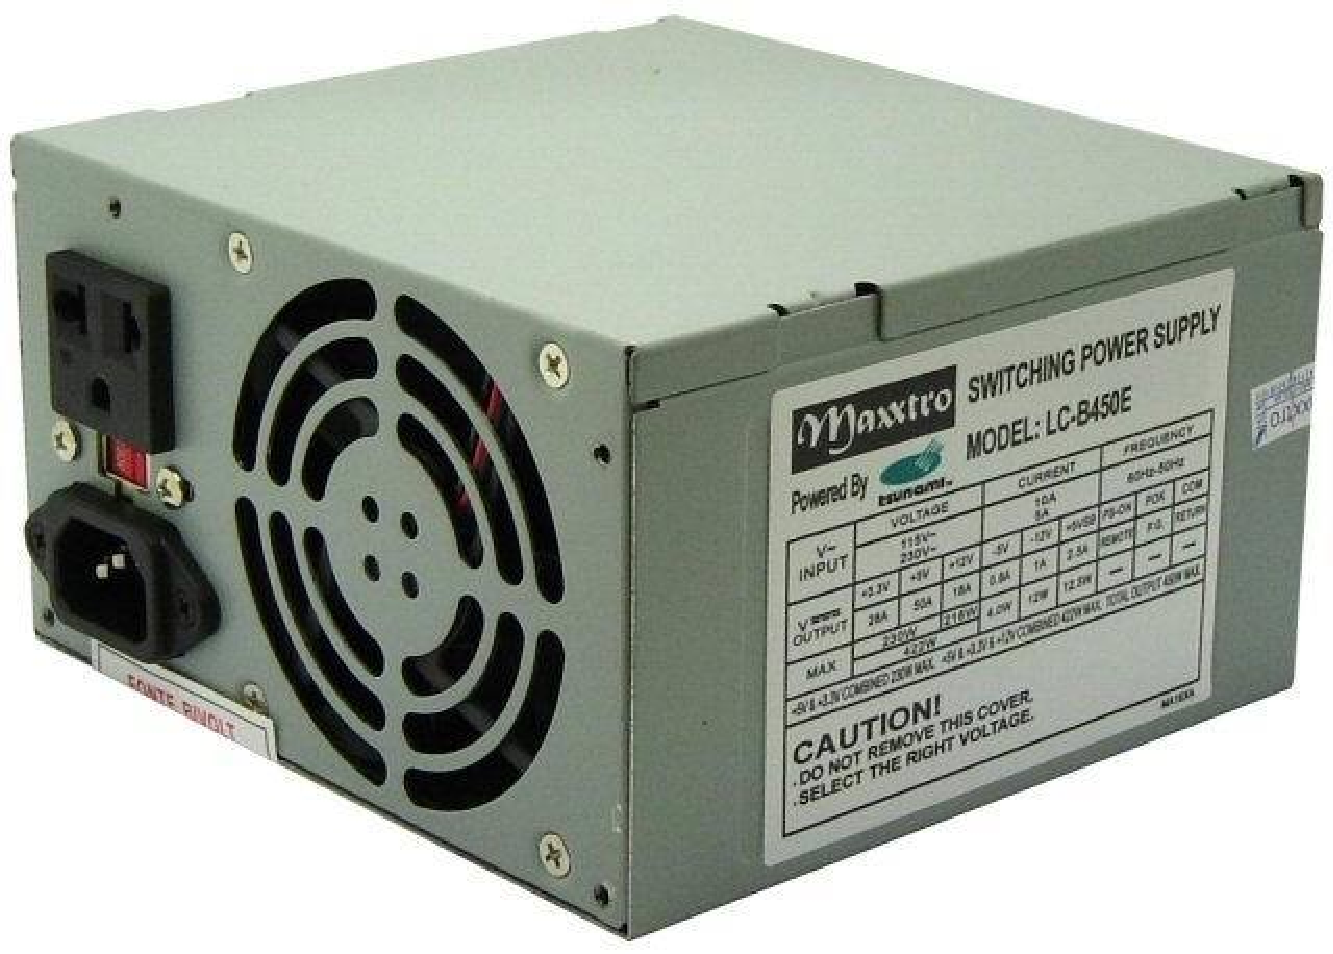
\includegraphics[scale=0.4]{figuras/fonte.pdf}
	\caption{A fonte de tensão pôde ser substituída pela fonte de computador descartado.}  \label{fig:fonte} 
\end{figure}

A fonte ilustrada pela figura \ref{fig:fonte} possui saídas de $12V$, $5V$, e $3,3V$, que podem ser combinadas em série para formar a tensão desejada. Com isso, \textit{podemos eliminar o uso da ponte retificadora, pois a fonte de computador já fornece corrente contínua}, conforme ilustra a figura \ref{fig:simulacao2}. A resistência fixa também não é necessária, já que vamos determinar a tensão fornecida pela fonte. A resistência variável pode ser substituída por um potenciômetro que, por \textit{divisor de tensão}, regulará a tensão aplicada ao banco de capacitores.
%
\begin{figure}[H]
	\centering
	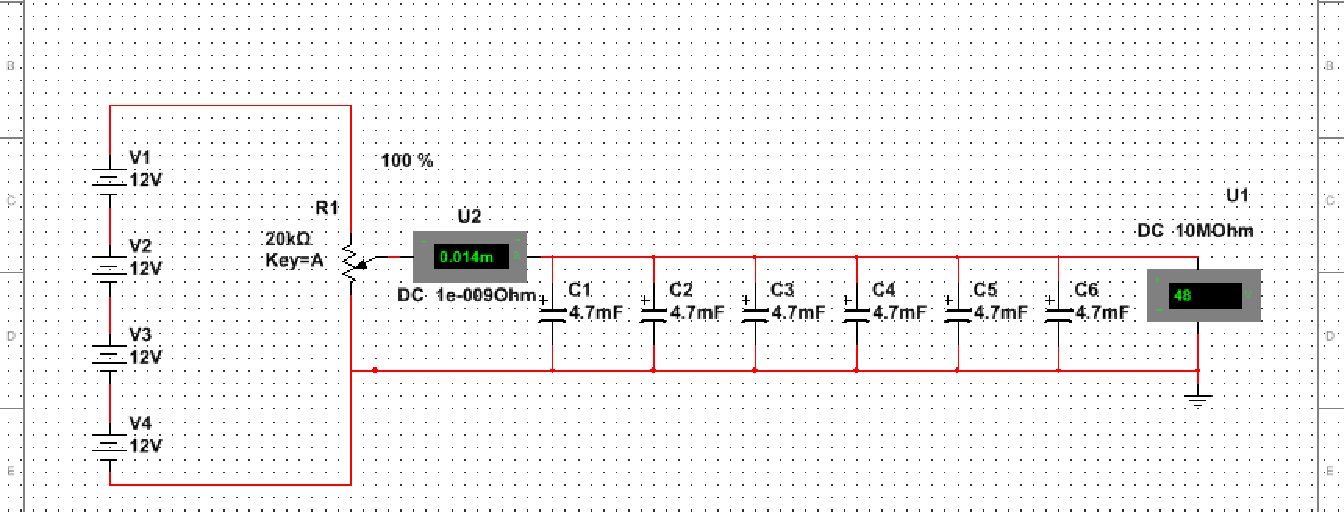
\includegraphics[scale=0.5]{figuras/simulacao2.pdf}
	\caption{Eliminando o uso da ponte retificadora ao utilizar a fonte de computador descartado.}  \label{fig:simulacao2} 
\end{figure}

Outra alternativa seria ligar um par de capacitores em série com outros pares em paralelo, dividindo assim a tensão aplicada em cada capacitor.
Como capacitores funcionam como circuito aberto (após carregados) em corrente contínua, utilizaremos uma ponte retificadora para converter CA em CC.

Utilizamos também uma resistência fixa de $35 \Omega$ $10 W$ e uma resistência variável de valor a definir para criar um divisor de tensão. O divisor de tensão é responsável por regular a tensão aplicada no banco de capacitores. Um voltímetro digital será usado no auxílio da aferição da tensão. 

Em outra atividade, alguns \textit{Totems}\footnote{Sistema computacional normalmente utilzado como caixas eletrônicos. Um totem é, em verdade, um sistema a eventos discretos, mais popularmente conhecido como autômato.} que se encontravam defeituosos, advindos de doações externas, foram montados e doados para diversos setores dentro da universidade, tais como a Mostra de profissões da UFOP, a Biblioteca da Escola de Minas, a diretoria da Escola de Minas e o Laboratório de Desenvolvimento de Novas Tecnologias e Prototipagem do DECAT-EM, conforme ilustra a figura \ref{fig:totem}.
\begin{figure}[H]
	\centering
	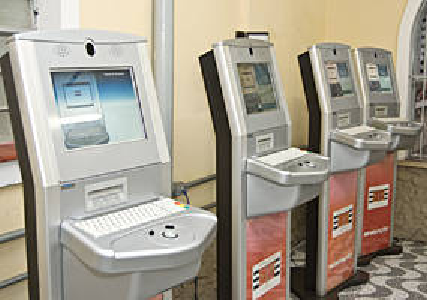
\includegraphics[scale=1.5]{figuras/totem.pdf}
	\caption{Totens recuperados (imagem ilustrativa).}  \label{fig:totem} 
\end{figure}


Na tabela \ref{tabela:manufatura} pode-se observar uma breve listagem com alguns dos componentes reciclados projeto Manufatura Reversa, até o mês de dezembro de $2016$.

\begin{table}[H]
	%\centering
	\caption{Relação de alguns dos materiais reciclados pelo projeto Manufatura Reversa}
	\label{tabela:manufatura}
\begin{tabular}{|l|l|l|l|}
	\hline
	\textbf{Código} & \textbf{Destino}              & \textbf{Material}         & \textbf{Quantidade} \\ \hline
	& Aluno Marco A. Reis           & Engrenagens de motores    & 2                   \\ \hline
	MR\_M\_001      & Decat                         & Monitor                   & 1                   \\ \hline
	MR\_M\_002      & Prof. Luís  Bartolaia         & Dissipadores              & 3                   \\ \hline
	MR\_M\_003      & Prof. Ronílson Decat          & Memórias 1gb DDR          & 2                   \\ \hline
	MR\_M\_004      & Prof. Ronílson Decat          & Placa mãe com processador & 2                   \\ \hline
	MR\_M\_005      & Prof. Ronílson Decat          & Fonte                     & 2                   \\ \hline
	MR\_M\_006      & Prof. Ronílson Decat          & Placa de vídeo 6200GT     & 1                   \\ \hline
	MR\_M\_007      & Biblioteca da Escola de Minas & totem                     & 2                   \\ \hline
	MR\_M\_008      & Mostra de profissões          & totem                     & 2                   \\ \hline
	MR\_M\_009      & Laboratório de prototipagem   & totem                     & 1                   \\ \hline
	MR\_M\_010      & Diretoria da Escola de Minas  & totem                     & 2                   \\ \hline
	MR\_M\_011      & Laboratório de usinagem       & fonte                     & 1                   \\ \hline
	MR\_M\_012      & Laboratório de usinagem       & capacitores               & 6                   \\ \hline
	MR\_M\_013      & Laboratório de usinagem       & Placas-mãe                & 2                   \\ \hline
	MR\_M\_014      & Laboratório de usinagem       & conectores                & diversos            \\ \hline
\end{tabular}
\end{table}

\section{Resultados do ``Frankenstein''}
Durante o projeto, foi possível realizar uma doação de um lote de onze computadores à instituição ``Casa Espírita Irmão Horta'' localizada na cidade de Mariana/MG. A instituição desenvolve ações educativas como organização não-governamental.

Cada um dos onze \textit{kits} era composto por: computador com processador Intel Dual Core, disco rígido de 80GB ou 160GB, memória RAM de 1GB, mouse P2, teclado P2, monitor LCD de 17", dois cabos de energia e um cabo VGA. Foi doado também um \textit{switch industrial} para possibilitar a montagem de uma rede de comunicação. 
\begin{figure}[H]
 		\centering
 		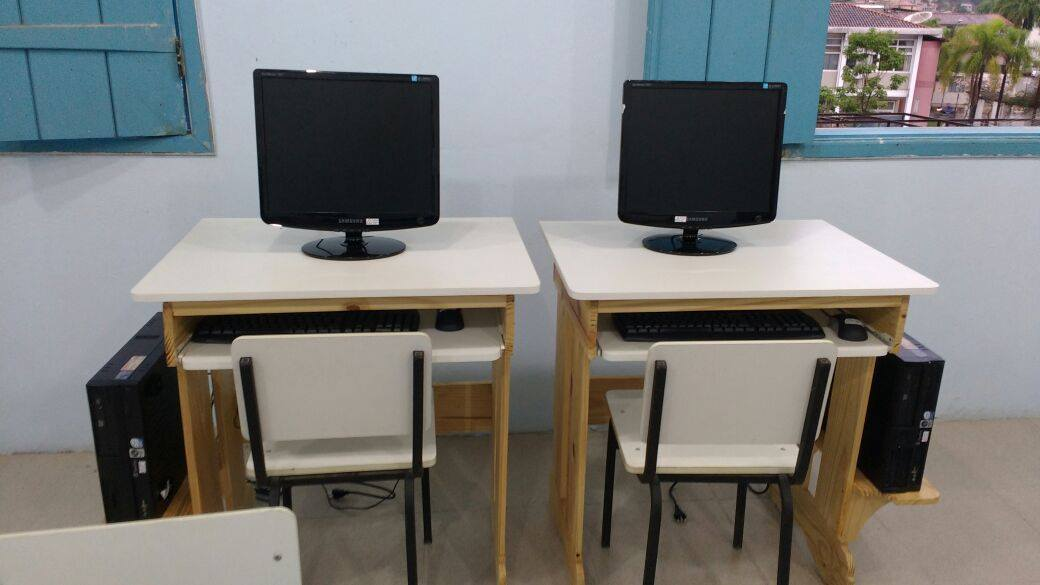
\includegraphics[scale=0.3,angle=0]{figuras/CasaEspirita1.jpg}
 		\caption{Laboratório da Casa Espírita Irmão Horta.}  \label{fig:CasaEspirita1} 
 		\end{figure} 

\begin{figure}[H]
 		\centering
 		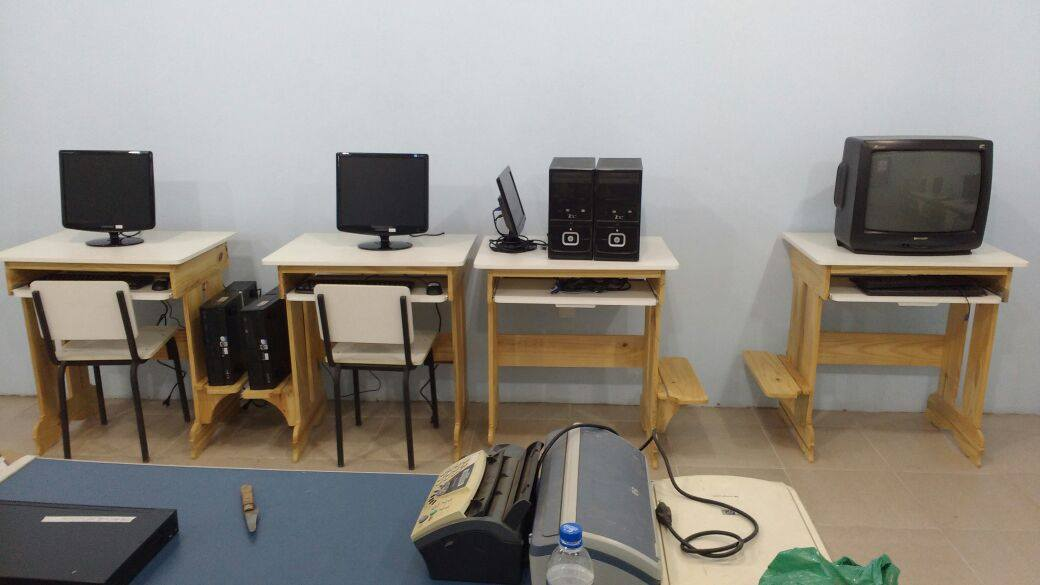
\includegraphics[scale=0.3,angle=0]{figuras/CasaEspirita2.jpg}
 		\caption{Laboratório da Casa Espírita Irmão Horta.}  \label{fig:CasaEspirita2} 
 		\end{figure} 

\begin{figure}[H]
 		\centering
 		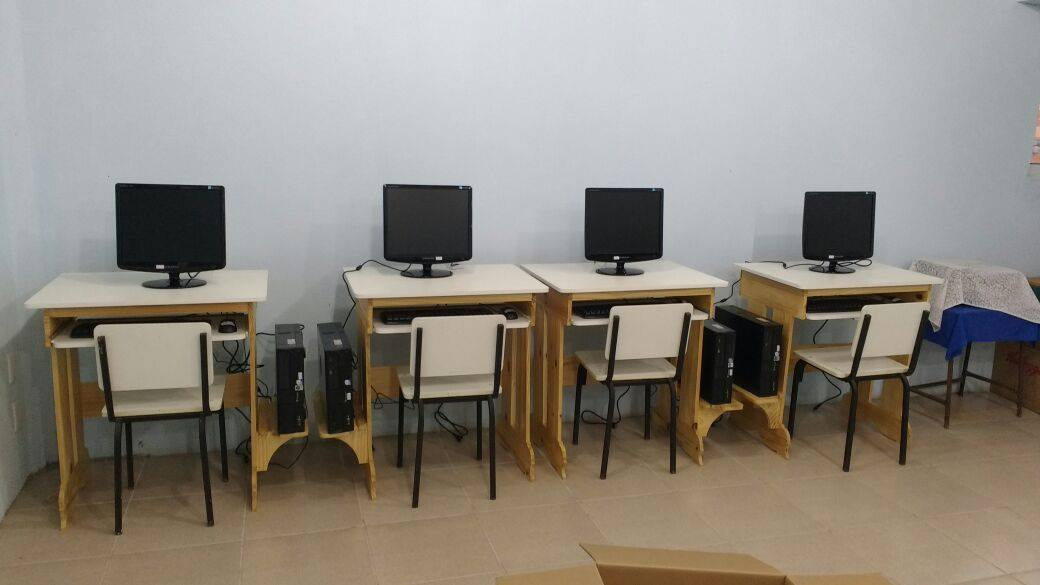
\includegraphics[scale=0.3,angle=0]{figuras/CasaEspirita3.jpg}
 		\caption{Laboratório da Casa Espírita Irmão Horta.}  \label{fig:CasaEspirita3} 
 		\end{figure} 

\begin{figure}[H]
 		\centering
 		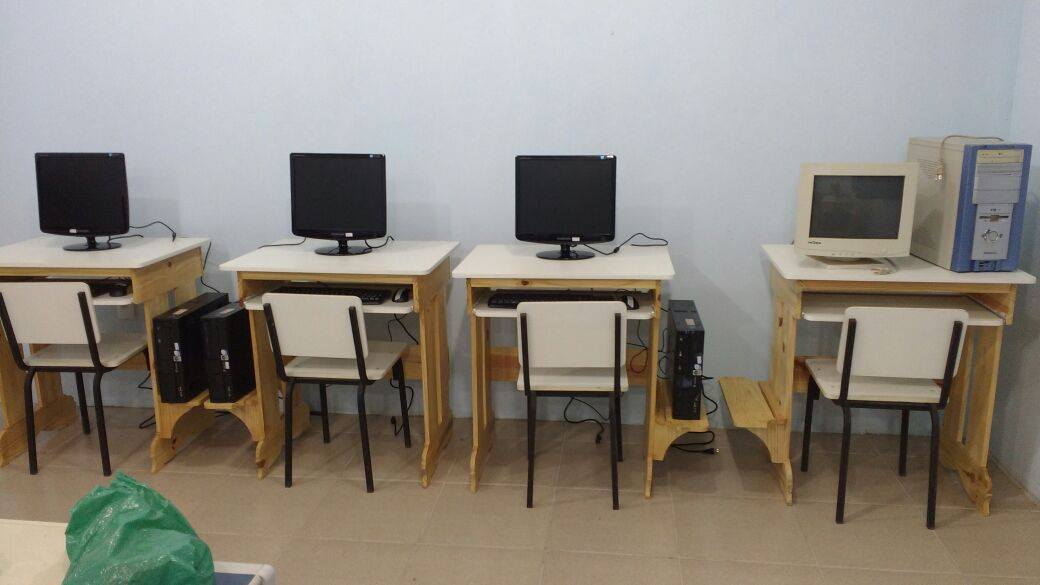
\includegraphics[scale=0.3,angle=0]{figuras/CasaEspirita4.jpg}
 		\caption{Laboratório da Casa Espírita Irmão Horta.}  \label{fig:CasaEspirita4} 
 		\end{figure} 

Além disso, os bolsistas tiveram a oportunidade de aprimorar os conhecimentos em manutenção de hardware e software de computadores.  
A falta de material para manutenção das máquinas, principalmente memória RAM, e o número reduzido de bolsistas prejudicou o andamento do projeto. Inicialmente o projeto contava com um bolsista e um voluntário mas o aluno voluntário ficou apenas um mês no projeto.  

% ---
% Conclusão
% ---
\chapter{Considerações Finais}

Foi possível observar durante o período de vigência do programa ``Reciclagem Digital'' que muitas tarefas foram realizadas. O projeto seguiu uma curva de aprendizagem que foi bastante satisfatória para atingir os seus objetivos. Em cada um dos três projetos (Frankestein, Manufatura Reversa e Hospital das Máquinas) foi possível perceber essa curva de aprendizagem.

Por ter se tratado de um programa novo, onde os integrantes ainda não tinham muita experiência, muito foi descoberto com o passar do tempo. Todos os desafios que apareceram foram superados de forma produtiva e o desempenho de toda a equipe sempre esteve satisfatório.

Por se tratar de uma equipe que ``abraça a causa'' do programa Reciclagem Digital, os resultados foram alcançados e as barreiras que apareceram foram superadas. Todas as etapas do programa foram executadas pensando no longo prazo, pois a ideia é que o projeto cresça e se amplie há cada ano, atingindo, com o passar do tempo, um maior número de pessoas atendidas por esse programa e também  aumentando o número de colaboradores na equipe.

% ---

% ----------------------------------------------------------
% ELEMENTOS PÓS-TEXTUAIS
% ----------------------------------------------------------
\postextual

% ----------------------------------------------------------
% Referências bibliográficas
% ----------------------------------------------------------
\bibliography{abntex2-modelo-references}

% ----------------------------------------------------------
% Glossário
% ----------------------------------------------------------
%
% Consulte o manual da classe abntex2 para orientações sobre o glossário.
%
%\glossary

% ----------------------------------------------------------
% Apêndices
% ----------------------------------------------------------

% ---
% Inicia os apêndices
% ---
\begin{apendicesenv}

% Imprime uma página indicando o início dos apêndices
\partapendices

% ----------------------------------------------------------
\chapter{Modelo de organograma} \label{ape:organograma}
% ----------------------------------------------------------
Como o programa buscou trabalhar desde seu início de uma forma colaborativa e, de certa forma, interdependente, uma proposta inédita para organização foi pensada de forma a gerenciar suas atividades. A partir desta proposta surgiu um novo modelo de organograma, que chamamos de ``organograma orbital''. A intenção é suprimir as dificuldades visuais e de intrepretação existentes em um organograma tradicional, que mostra apenas relações de verticalidade e horizontalidade. Como tínhamos no início diversos coordenadores de projeto que se interconunicavam e gerenciavam, ao mesmo tempo, as atividades dos bolsistas de todos os projetos, foi imaginado como cada bolsista poderia transitar entre os diferentes afazeres e, além disso, como se daria a comunicação entre eles e os coordenadores, que também realizam tarefas similares aos alunos. Daí concebeu-se a ideia do organograma orbital, conforme ilustra a figura \ref{fig:organograma} 

Cada planeta representa um coordenador de equipe. Cada satélite, que gira ao redor dos planetas, tem a primeira função de atender ao projeto vinculado, mas compartilha, por outro lado, a  mesma órbita de outros planetas, o que mostra que eles possuem funções diversas além da primeira (os nomes entre parênteses podem representar os alunos voluntários com a mesma função que o ``satélite''). Ao redor da ``estrela'' orbita um ``cometa'', personificado pelo bolsista de gerenciamento de projetos, que transita mais livremente entre todos. A sua órbita elíptica, aliás, indica uma maior proximidade em relação a um projeto em detrimento aos outros.

As setas indicam uma via de comunicação horizontal, lembrando que um sistema solar encontra-se em determinado plano do espaço. Isto é, todos os elementos são essenciais para o funcionamento do sistema como um todo e não existe hierarquia de verticalidade conforme a conhecemos, embora existam figuras centrais. Apenas relações de colaboração e interdependência, assim como a atração gravitacional exercida por cada astro em um sistema solar real.  	   
\begin{figure}[H]
 		\centering
 		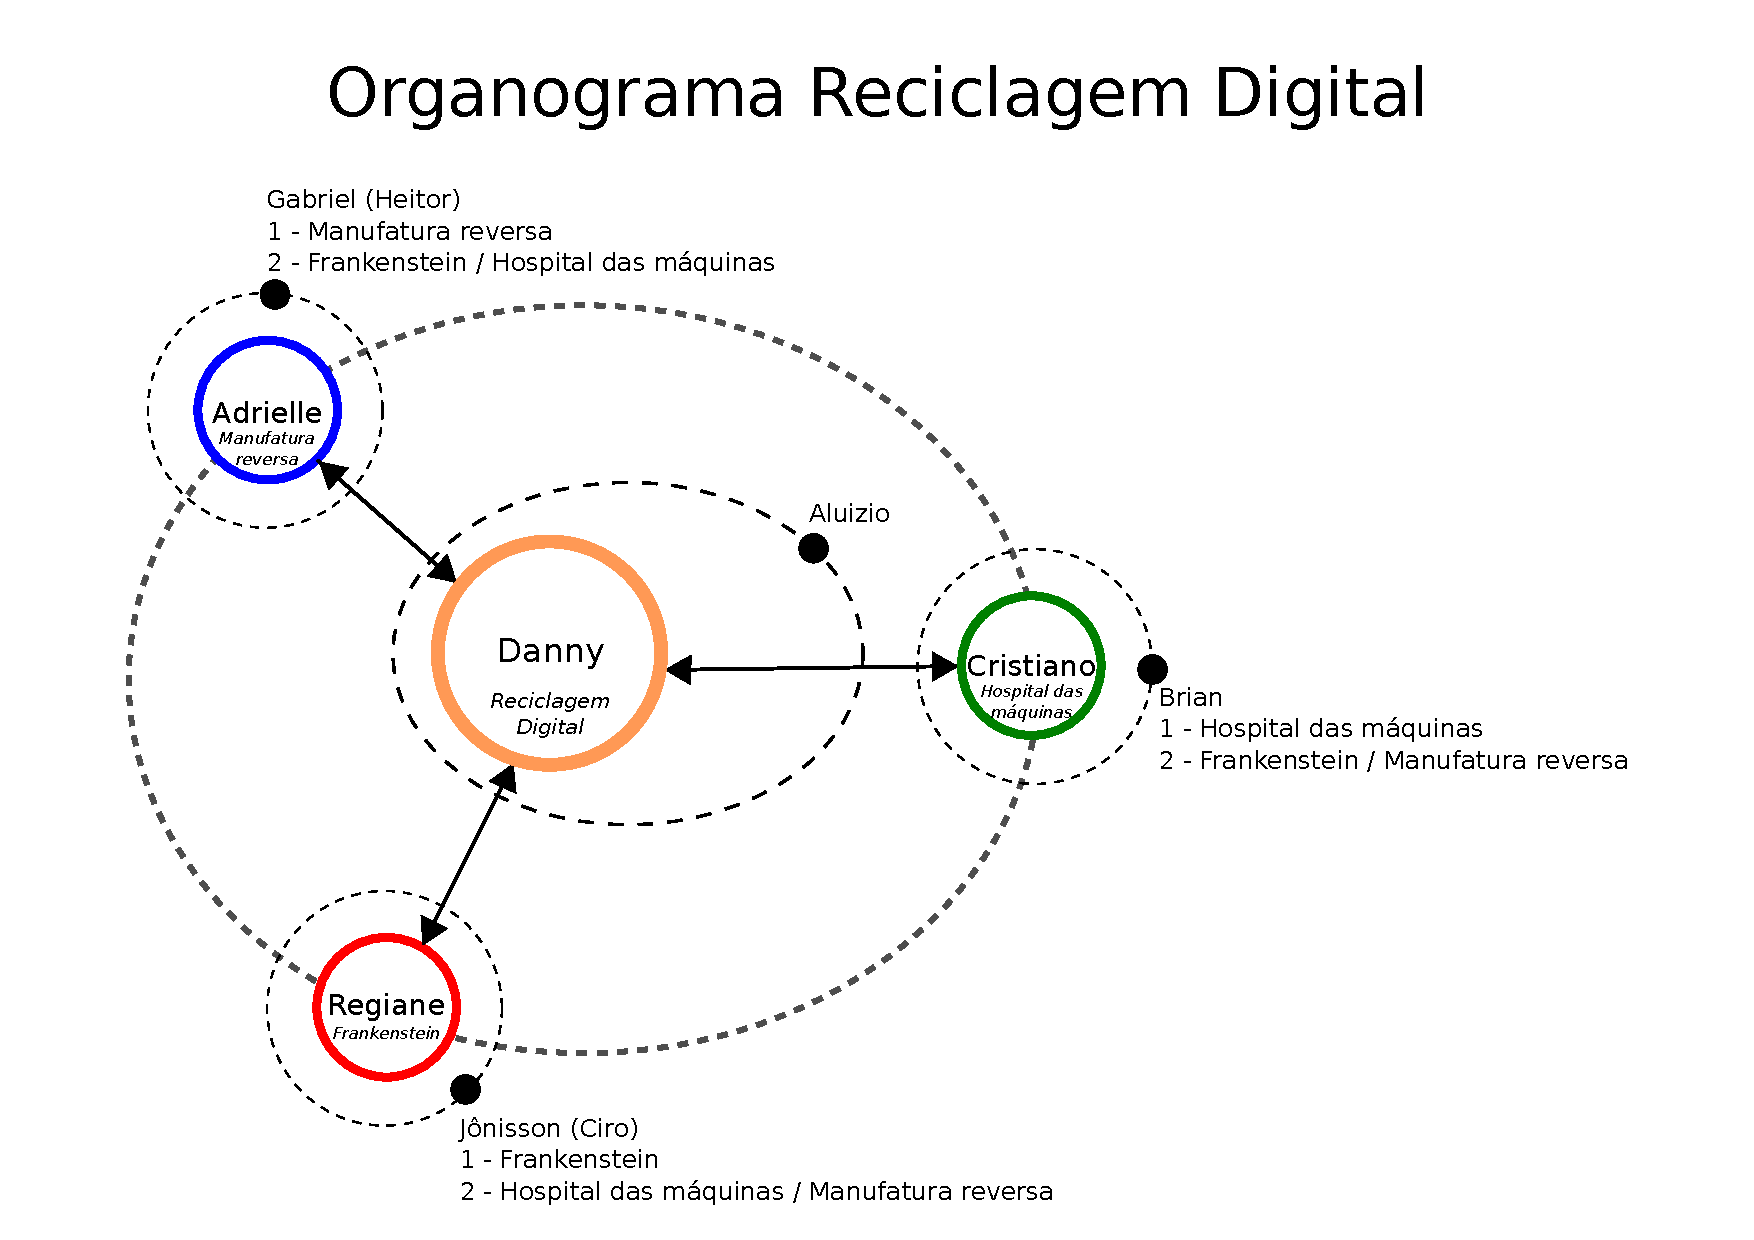
\includegraphics[scale=0.8,angle=90]{figuras/organograma.pdf}
 		\caption{Proposta de modelo de organização.}  \label{fig:organograma} 
 		\end{figure} 
% ----------------------------------------------------------
\chapter{Desenvolvimento de Logomarca}
% ----------------------------------------------------------
\begin{figure}[H]
	\centering
	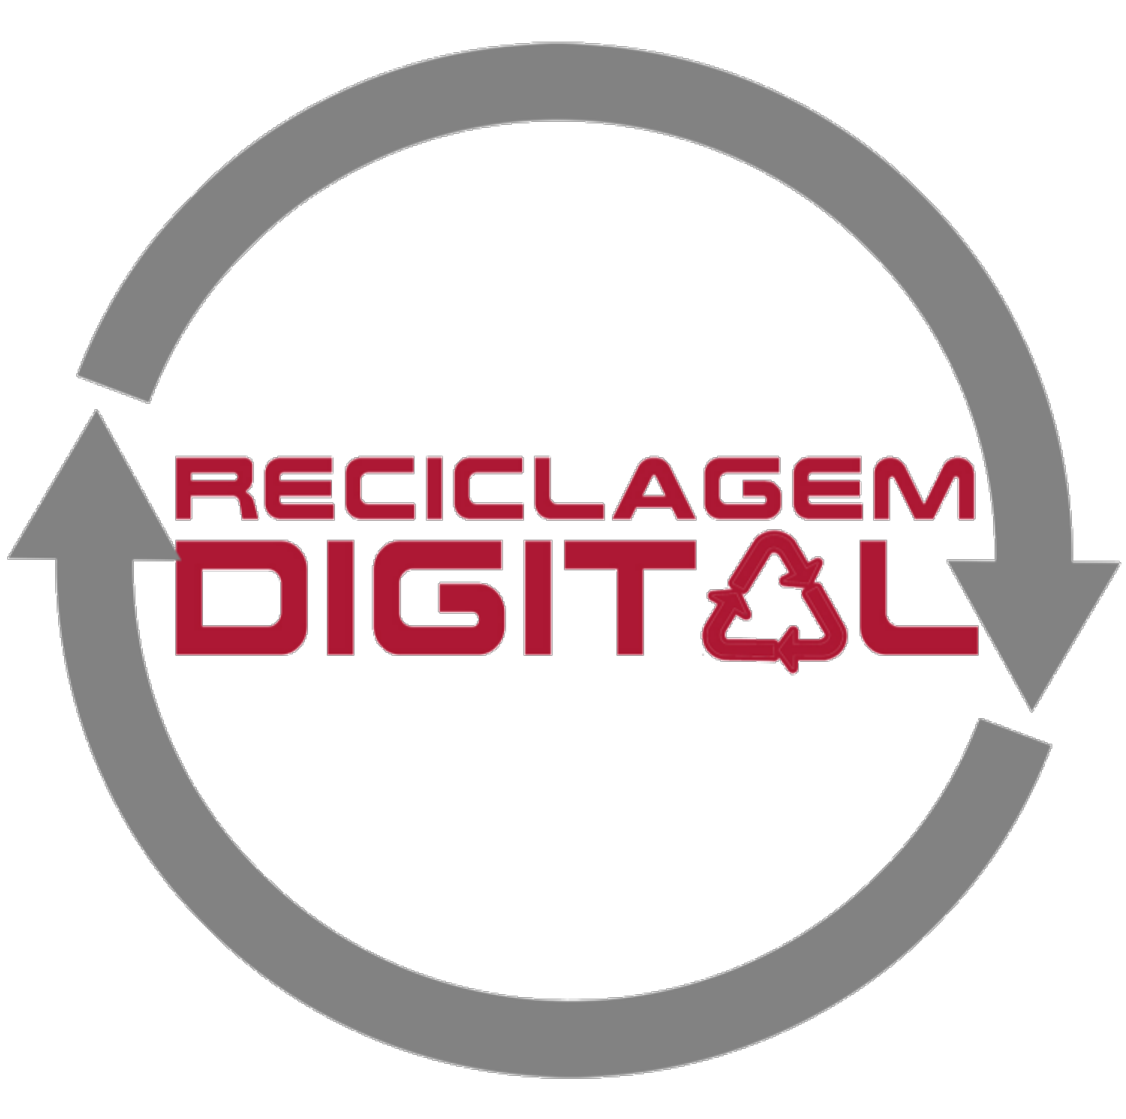
\includegraphics[scale=0.5]{figuras/logo-atual-reciclagem-digital-transparente.pdf}
	\caption{Logomarca do Reciclagem Digital.} \label{fig:logo} 
\end{figure}

% ----------------------------------------------------------
\chapter{Material de divulgação impresso}
% ----------------------------------------------------------
\begin{figure}
	\centering
	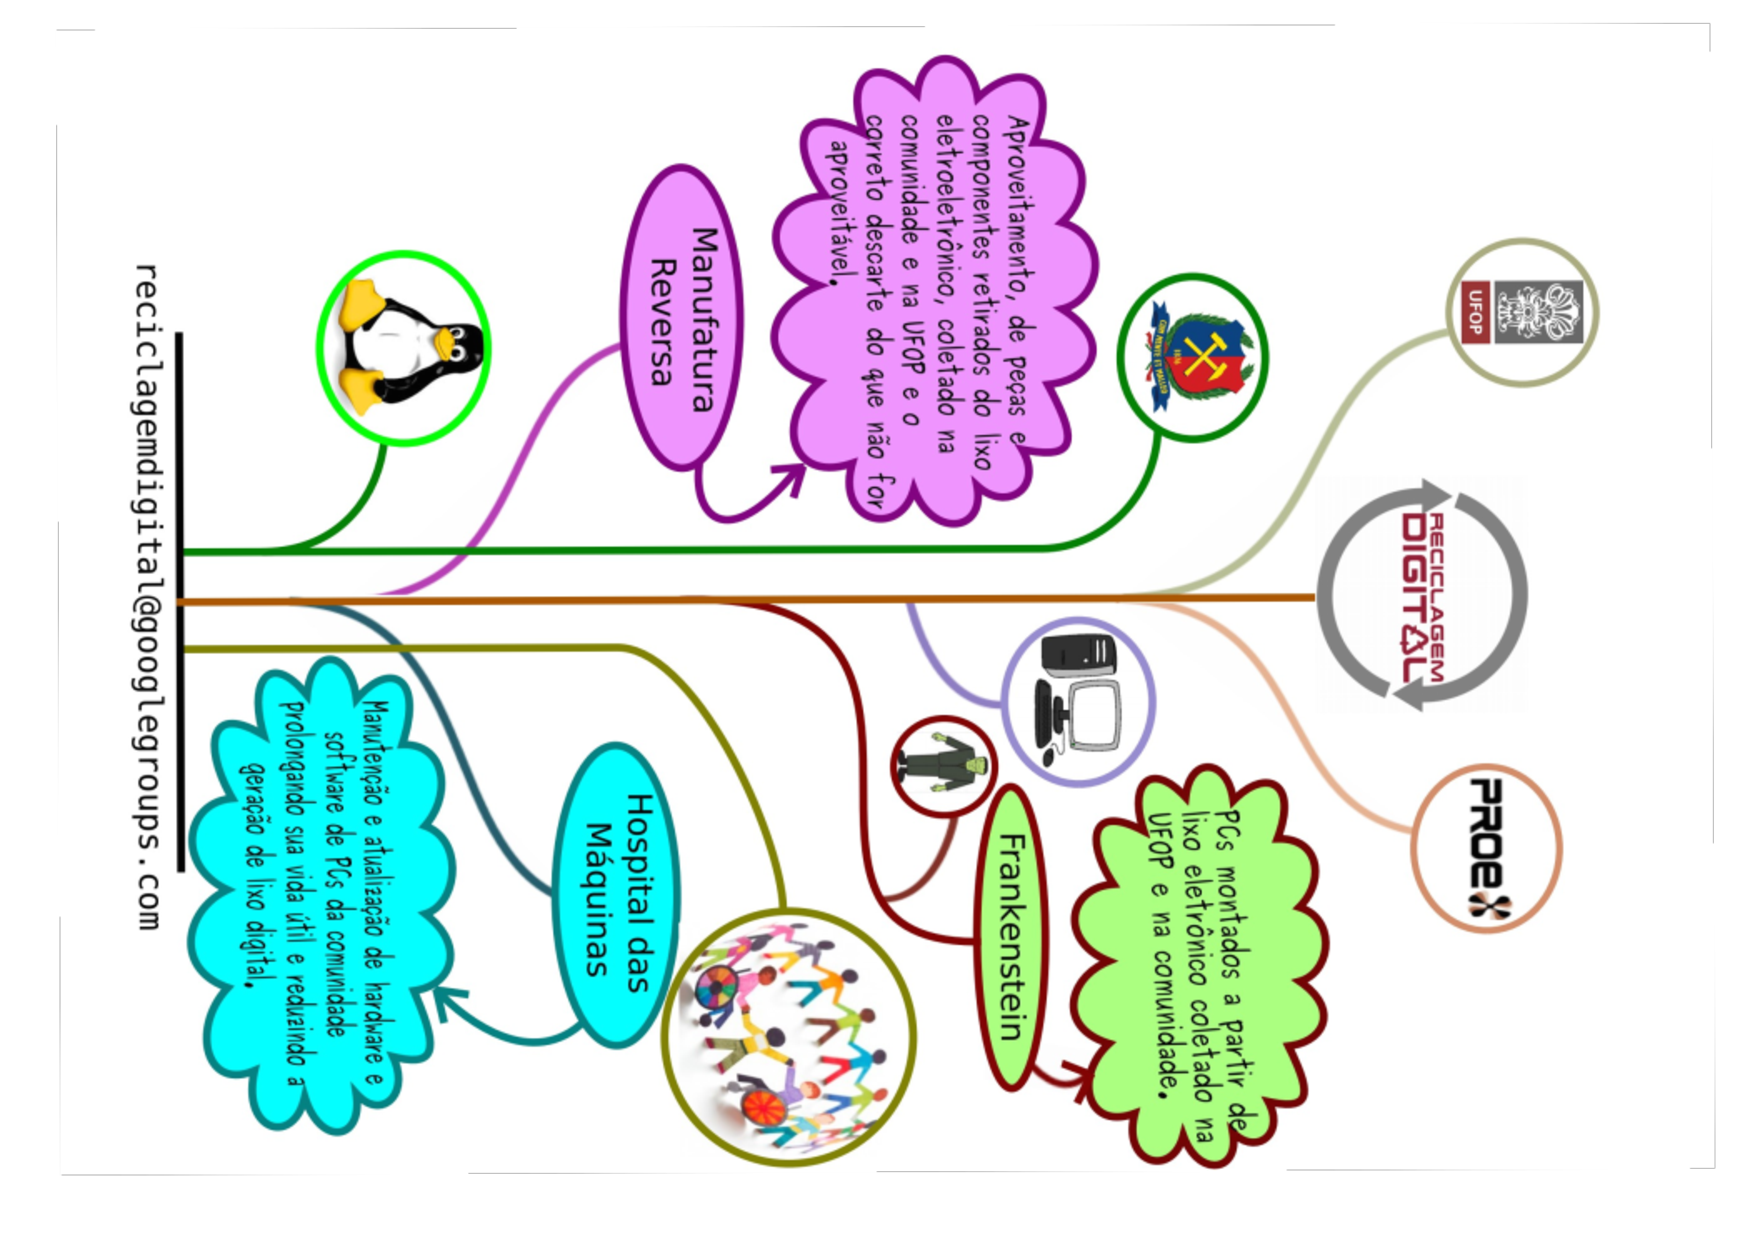
\includegraphics[scale=0.8,angle=90, scale=0.5]{figuras/panfleto.pdf}
	\caption{Primeiro material de divulgação impresso.}  \label{fig:divulgacao} 
\end{figure} 
% ----------------------------------------------------------
\chapter{Ordem de serviço}
% ----------------------------------------------------------
Em todas as instituições visitadas, um comprovante com a ordem de serviço era emitida, conforme ilustra a figura \ref{ordem-servico}. Vale ressaltar que a logomar utilzada não é mais a mostrada, pois contradizia o regimento da ufop. Vide o apêndice \ref{anexo:logomarca}.
\begin{figure}
	\centering
	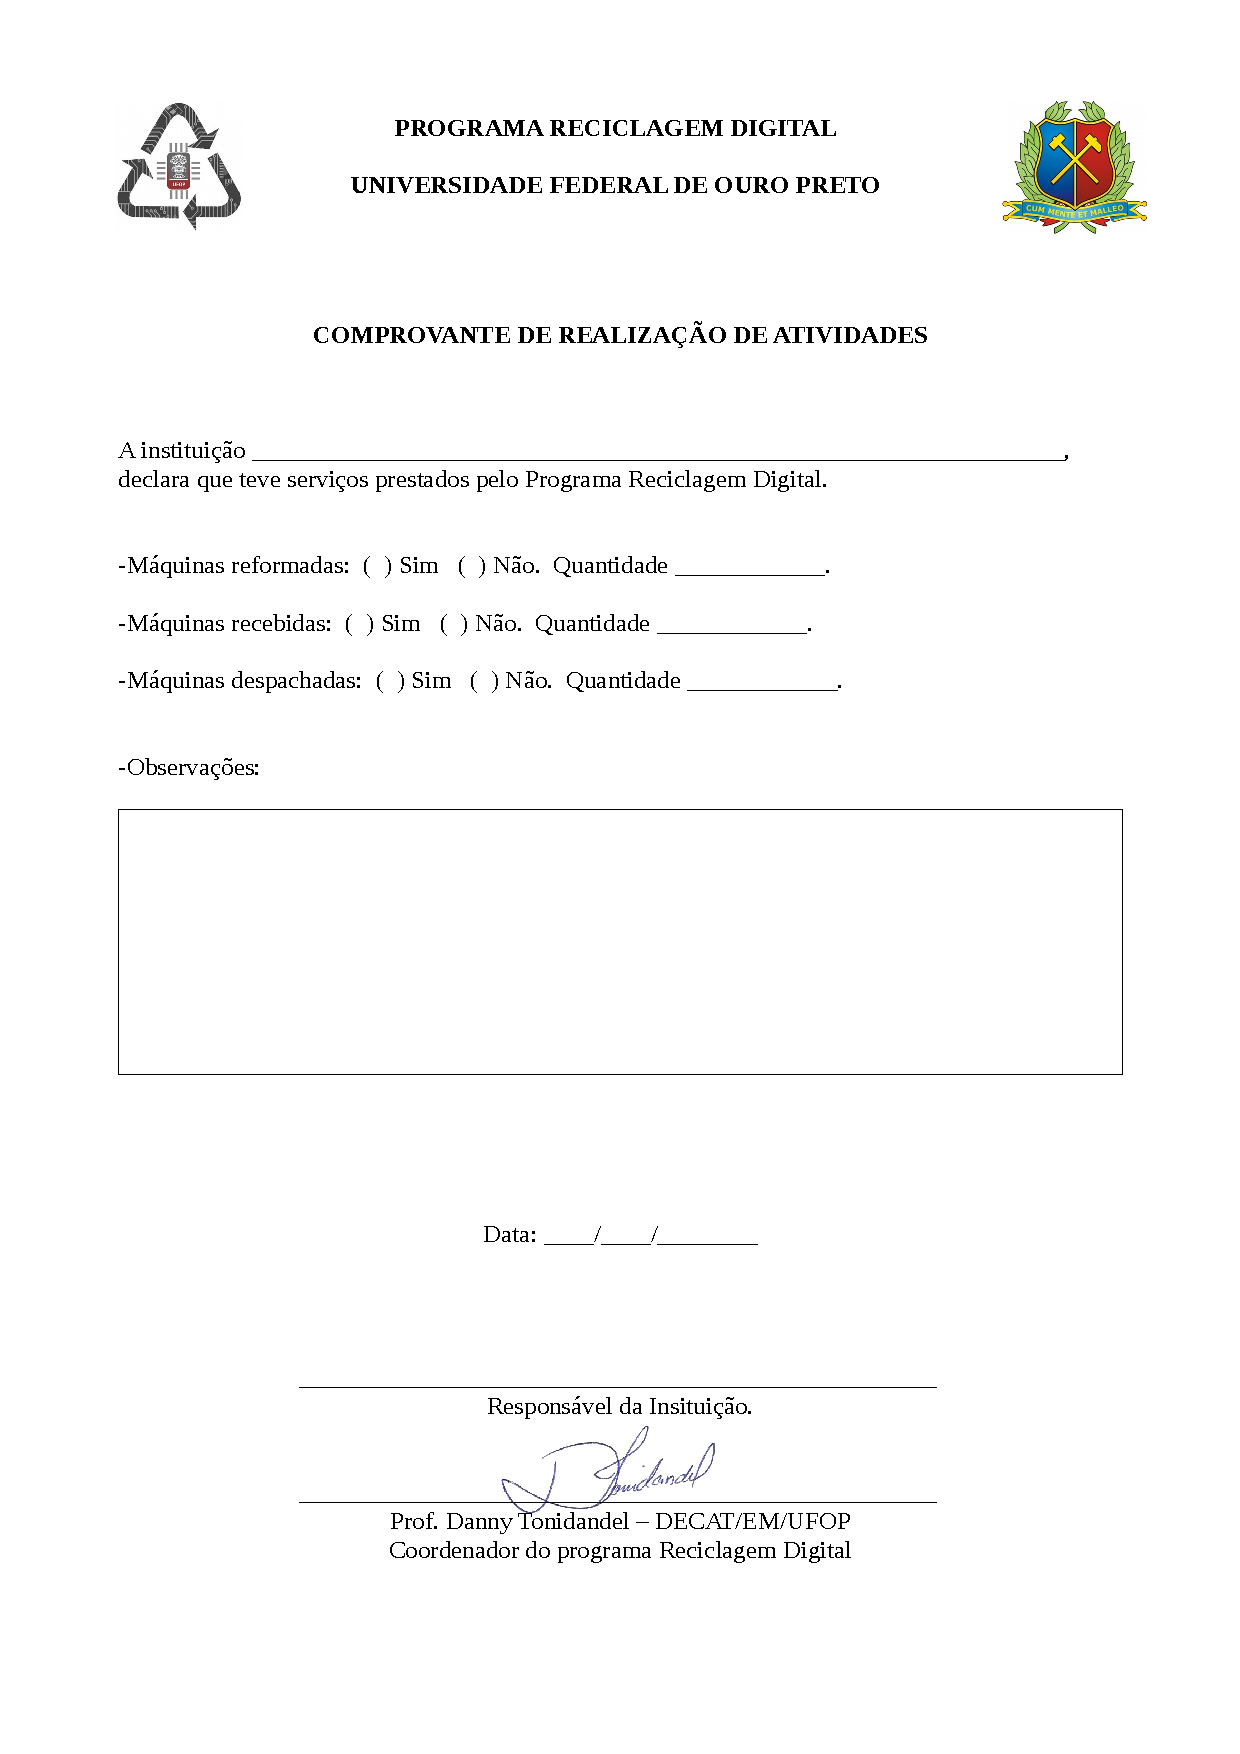
\includegraphics[scale=0.7]{figuras/comprovante-servico.pdf} 
	\caption{Ordem de serviço.}
	\label{ordem-servico}
\end{figure} 

% ----------------------------------------------------------
\chapter{Estoque de ferramentas}
% ----------------------------------------------------------
Uma listagem de ferramentas (adquirida \textbf{com recursos próprios dos docentes} para o início do projeto) é mostrada na figura \ref{tabela:estoque}.

\begin{figure}
	\centering
	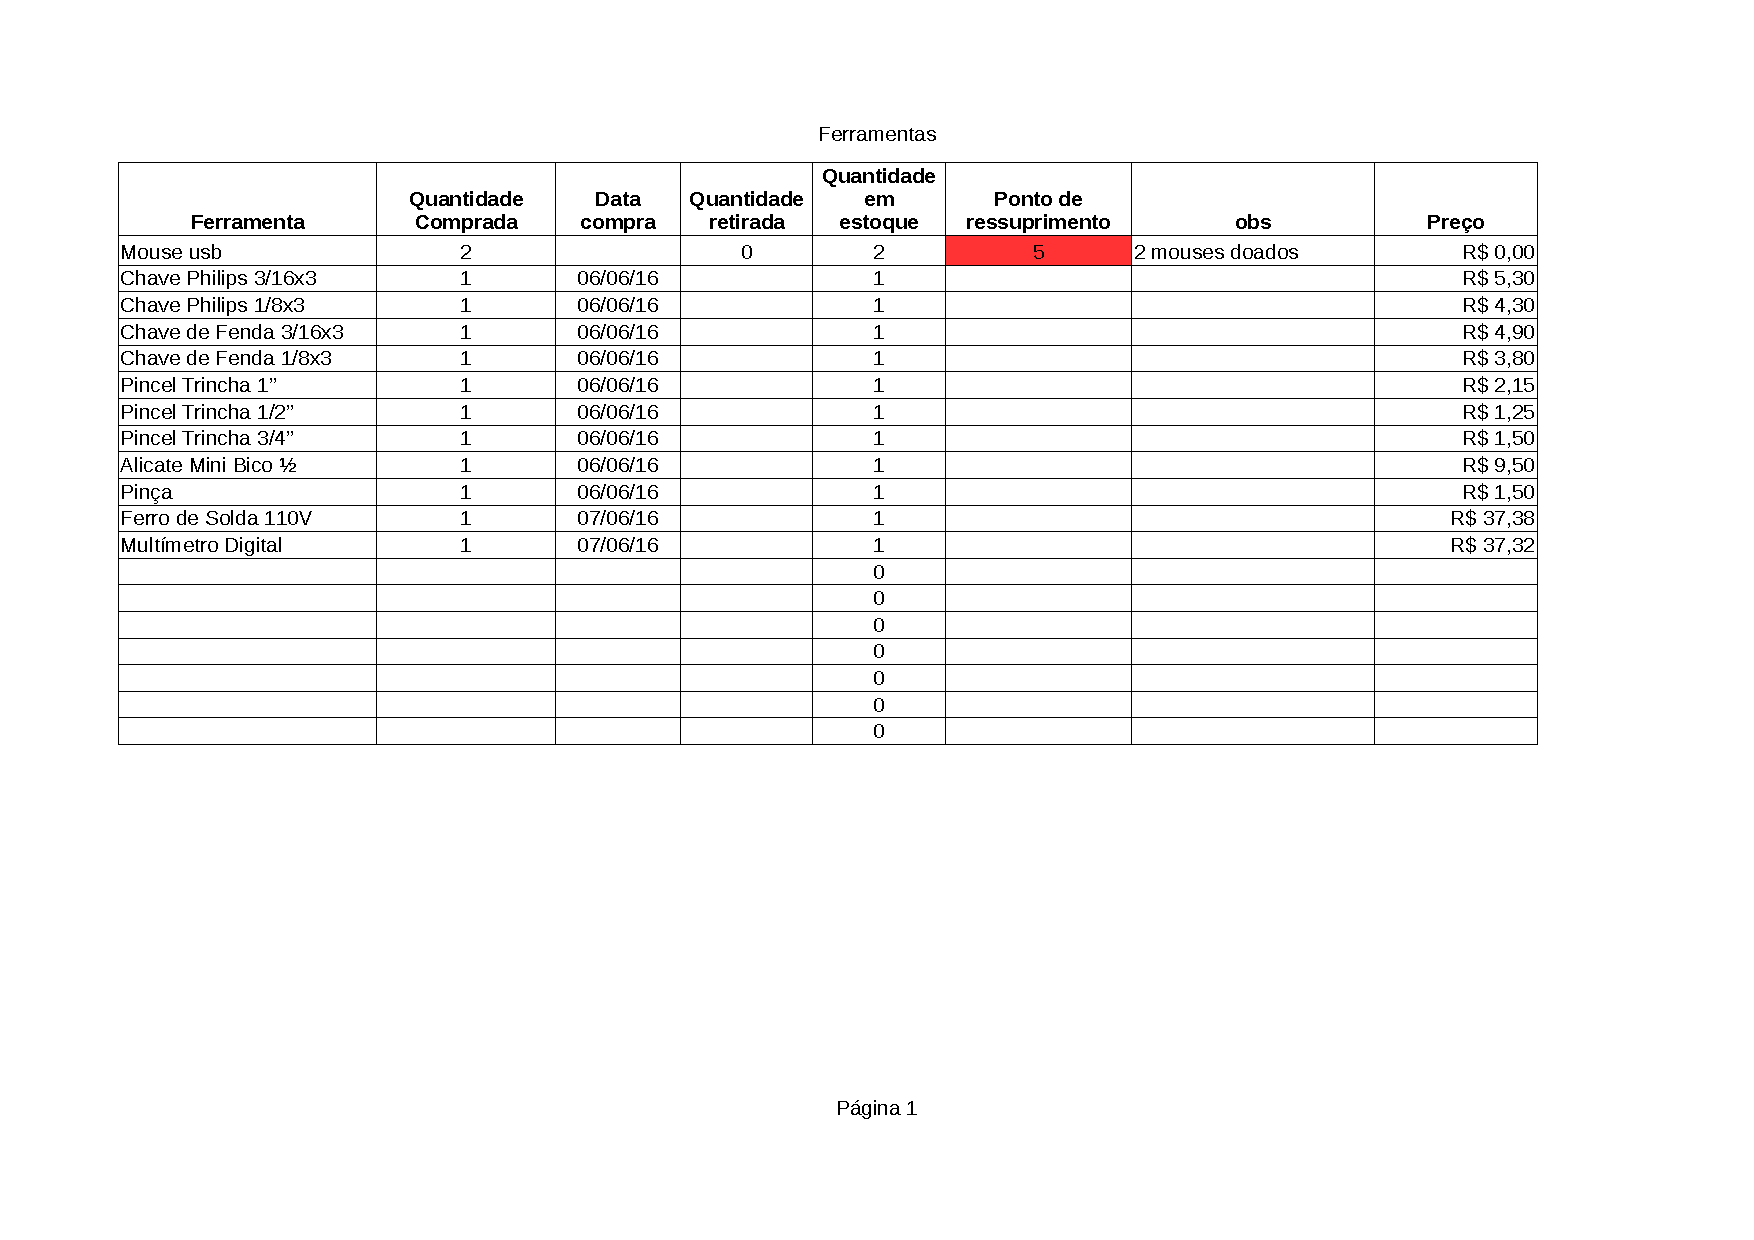
\includegraphics[scale=0.8, angle=90]{figuras/estoque-ferramentas.pdf} 
	\label{tabela:estoque}
	\caption{Listagem de ferramentas adquiridas com recursos dos docentes.}
\end{figure}

\end{apendicesenv}
% ---

% ----------------------------------------------------------
% Anexos
% ----------------------------------------------------------

% ---
% Inicia os anexos
% ---
\begin{anexosenv}

% Imprime uma página indicando o início dos anexos
\partanexos

%----- 
 \chapter{Matéria jornalística sobre o ``Reciclagem Digital''} \label{apendice:materia}
 %inserindo as páginas 1 e 2
 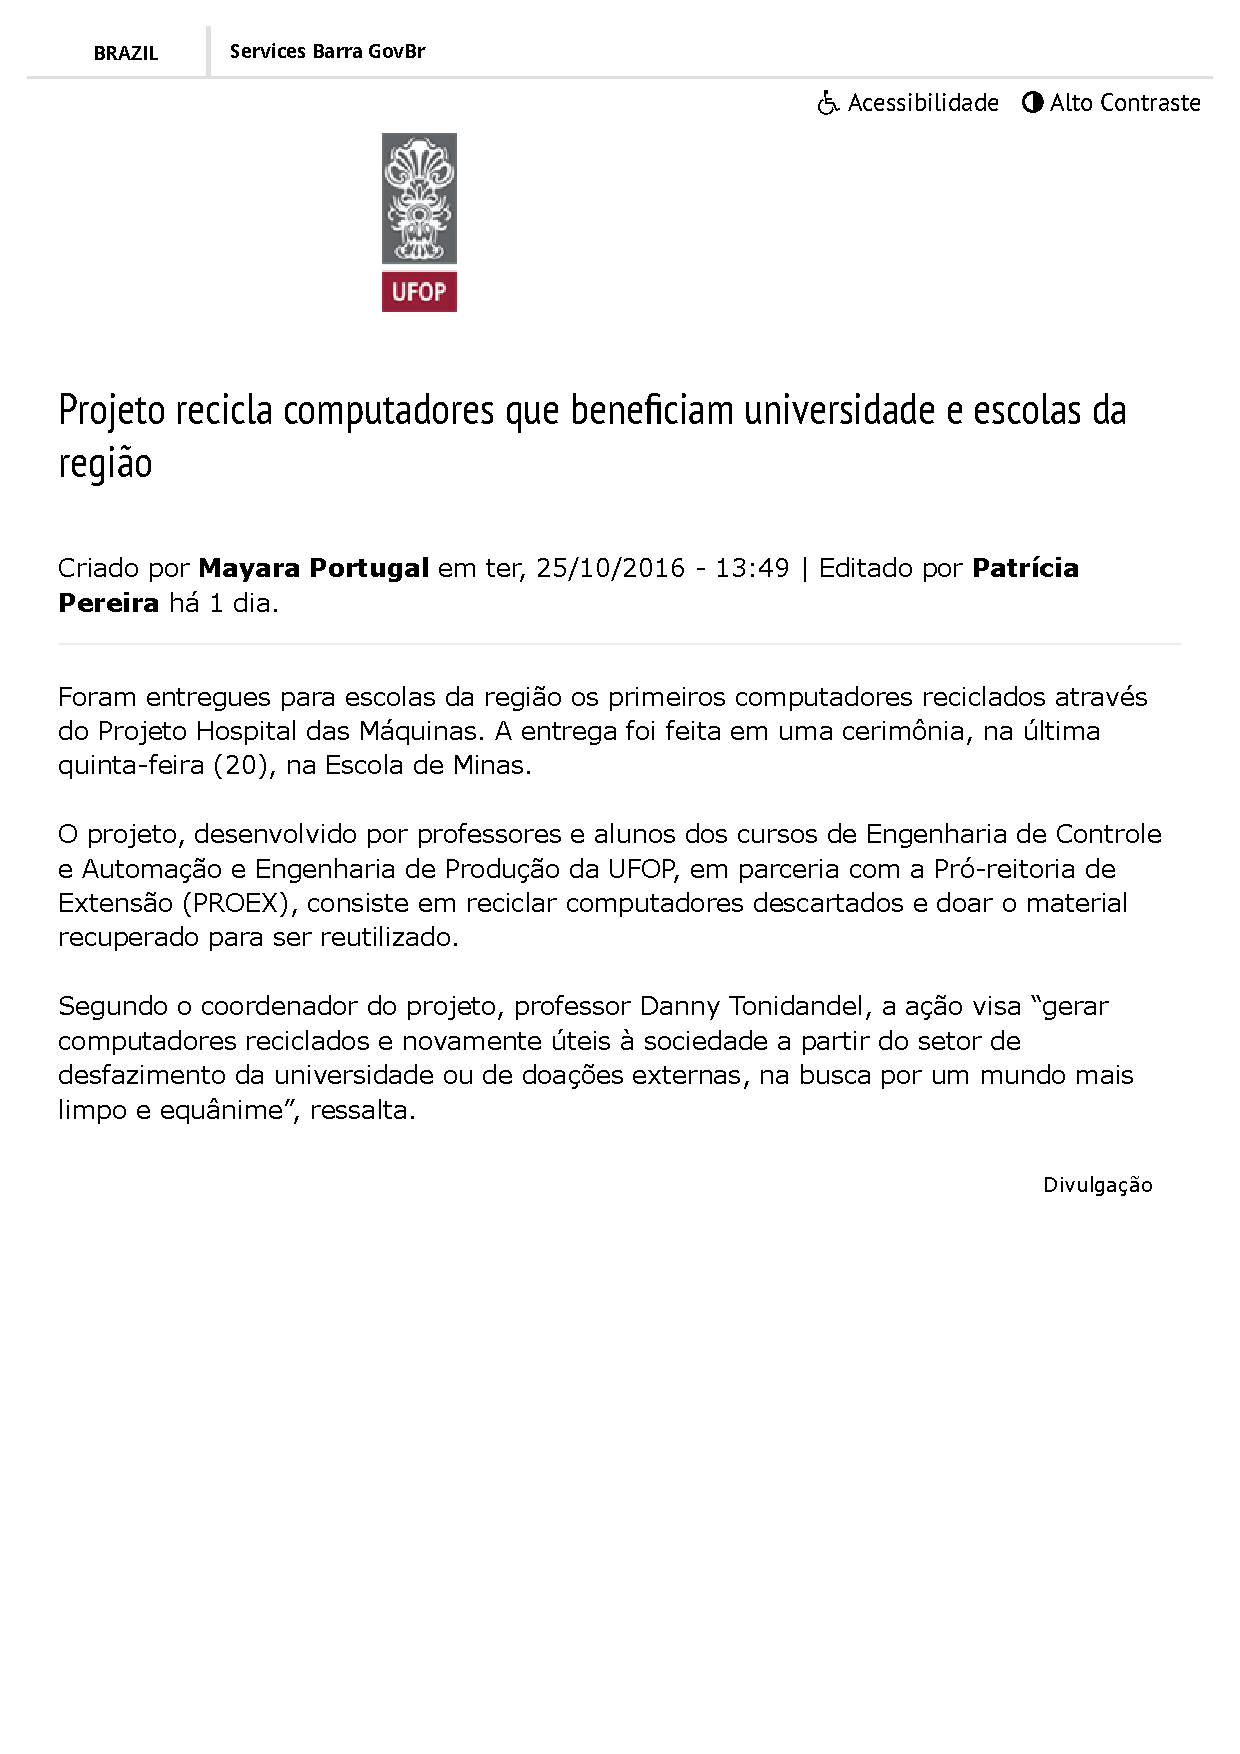
\includepdf[pages=1-2]{figuras/materia-site-ufop.pdf}	

\end{anexosenv}

\begin{comment}
%---------------------------------------------------------------------
% INDICE REMISSIVO
%---------------------------------------------------------------------

\phantompart

\printindex

%---------------------------------------------------------------------
% Formulário de Identificação (opcional)
%---------------------------------------------------------------------
\chapter*[Formulário de Identificação]{Formulário de Identificação}
\addcontentsline{toc}{chapter}{Exemplo de Formulário de Identificação}
\label{formulado-identificacao}

Exemplo de Formulário de Identificação, compatível com o Anexo A (informativo)
da ABNT NBR 10719:2015. Este formulário não é um anexo. Conforme definido na
norma, ele é o último elemento pós-textual e opcional do relatório.

\bigskip

\begin{tabular}{|p{9cm}|p{5cm}|}
\hline
\multicolumn{2}{|c|}{\textbf{\large Dados do Relatório Técnico e/ou científico}}\\
\hline
\multirow{4}{10cm}[24pt]{Título e subtítulo}& Classificação de segurança\\
                   & \\
                   \cline{2-2}
                   & No.\\
                   & \\
				
\hline
Tipo de relatório & Data\\
\hline
Título do projeto/programa/plano & No.\\
\hline
\multicolumn{2}{|l|}{Autor(es)} \\
\hline
\multicolumn{2}{|l|}{Instituição executora e endereço completo} \\
\hline
\multicolumn{2}{|l|}{Instituição patrocinadora e endereço completo} \\
\hline
\multicolumn{2}{|l|}{Resumo}\\[3cm]
\hline
\multicolumn{2}{|l|}{Palavras-chave/descritores}\\
\hline
\multicolumn{2}{|l|}{
Edição \hfill No. de páginas \hfill No. do volume \hfill Nº de classificação \phantom{XXXX}} \\
\hline
\multicolumn{2}{|l|}{
ISSN \hfill \hfill Tiragem \hfill Preço \phantom{XXXXXXXX}} \\
\hline
\multicolumn{2}{|l|}{Distribuidor} \\
\hline
\multicolumn{2}{|l|}{Observações/notas}\\[3cm]
\hline
\end{tabular}

\end{comment}
\end{document}
